\documentclass[a4j]{jarticle}
\usepackage[dvipdfmx]{graphicx}
\usepackage{amssymb}
\usepackage{amsmath}
\usepackage{subfigure}

\setlength\floatsep{0.2pt}
\setlength\abovecaptionskip{0.2pt}

\newcommand{\argmax}{\mathop{\rm arg~max}\limits}

\begin{document}
\begin{table}[t]
\begin{center}
{\large 産業用モニタリングシステムにおける障害検知手法の提案}\\
令和 2 年 8 月 28 日\\
山本 航平
\end{center}
\end{table}

進捗報告
\begin{itemize}
\item 一日を通じた計測実験で見られる,低遅延帯が時間経過に伴い増加傾向を示す区間の抽出に取り組んでいます.
\item FTP を併用した計測実験を行いました.(データはまだ見ていません)
\item 8 月 21 日(金)から 8 月 26 日(水)までの間,お貸しいただいた SIM を用いて一日を通じた計測を行いました.(データはまだ見ていません)
\end{itemize}

\section{実験設定}
一日を通した応答遅延の計測データを収集した.
機器構成は LTE モジュール として Quectel 社製 EC21-J を搭載した Raspberry Pi が NTT ドコモのキャリア回線を通じて一台の AWS サーバと接続されている.
また,LTE 回線としては IIJ モバイル社のサービスタイプ D 定額プランライト(いちねんプリペイド)を用いた.
応答遅延はこの Raspberry Pi から AWS サーバに対して ping コマンドを実行することで計測した.
ただし,ping はパケットサイズ60 バイト,ICMP ECHO メッセージ,パケット数 1 とする.
ping コマンドは 15 秒毎に実行するものとし,実行直前の時刻と組み合わせることで応答遅延の時系列データを得た.

\section{背景}
一日を通した計測結果の一部を図 \ref{rise} に示す.
この図は横軸を時刻とし,縦軸に対応する時刻に計測した ping 応答値をとった折れ線グラフである.
ただし赤色破線は LTE 接続が切れた時刻を表すが,ここでは取り扱わないので詳細は省く.
この図のように低遅延帯に分布する応答遅延が緩やかに増加していき,しばらくすると急激に減少して再度緩やかに増加していく傾向がみられる.
\begin{figure}[tb]
\begin{center}
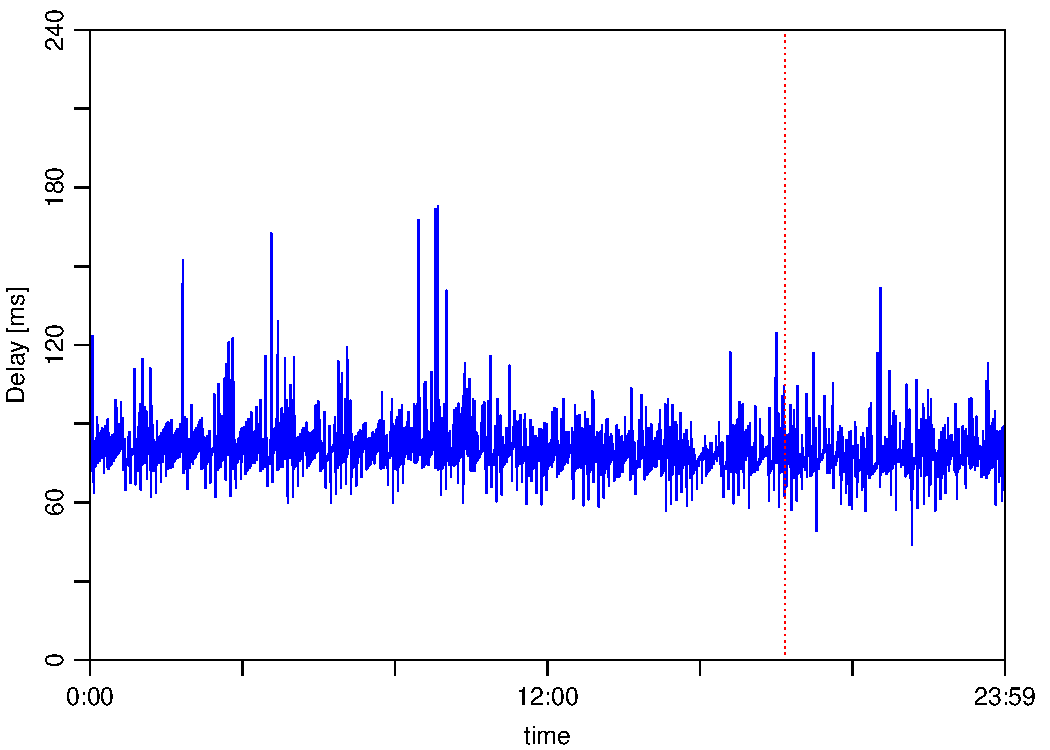
\includegraphics[width=\hsize]{C:/master/mstudy/analysis/long/plot-6-23.pdf}
\caption{6 月 23 日(火)に得られた応答遅延の時間データ}
\label{rise}
\end{center}
\end{figure}
この右肩上がりの傾向は図 \ref{otherrise} のように計測日に問わず見られることから,応答遅延の変動の仕方を特徴づけるものと考えられる.
\begin{figure}[tb]
\begin{center}
\subfigure[6 月 24 日(水)]{
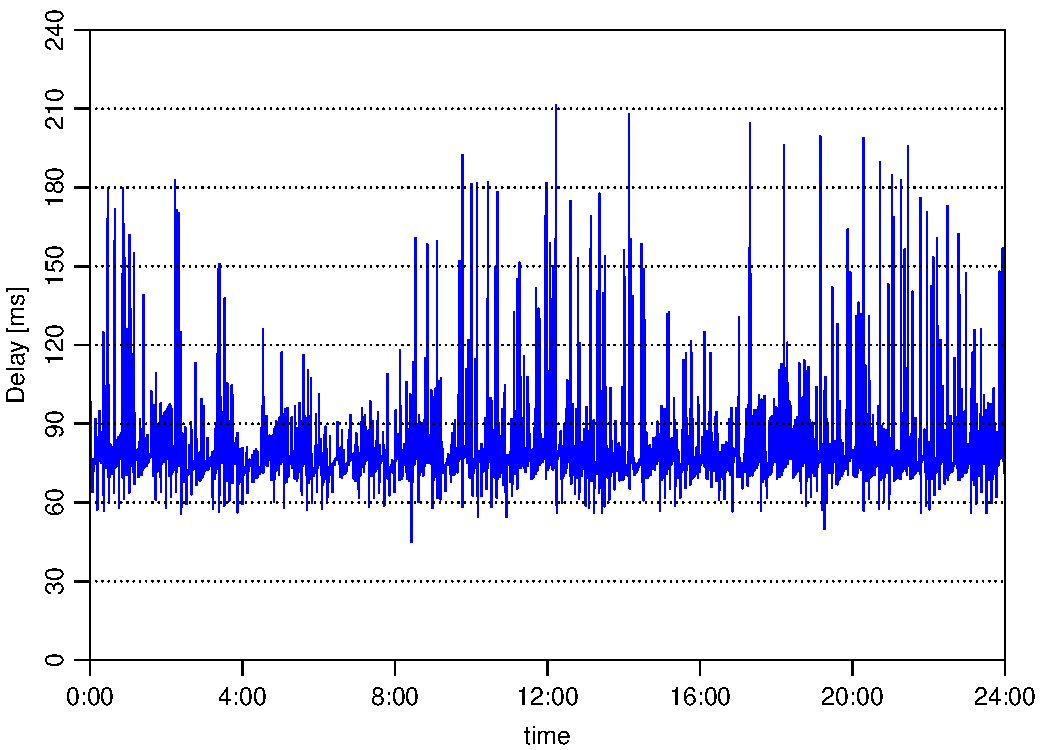
\includegraphics[width=0.5\hsize]{C:/master/mstudy/analysis/long/plot-6-24.pdf}
}~
\subfigure[6 月 25 日(木)]{
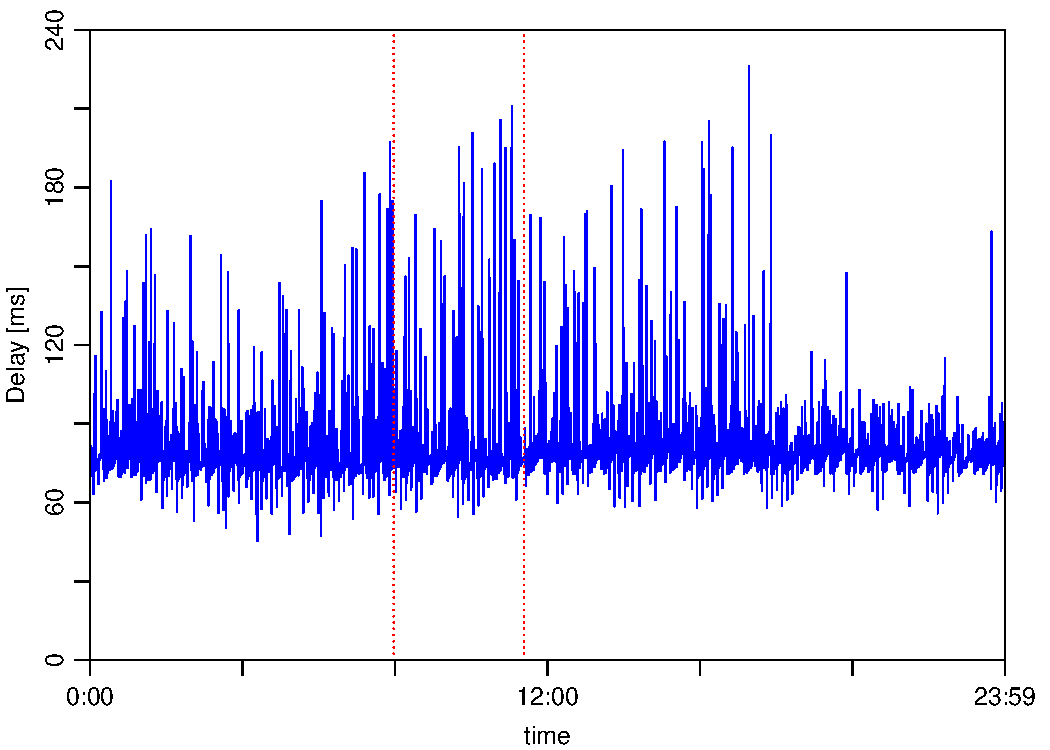
\includegraphics[width=0.5\hsize]{C:/master/mstudy/analysis/long/plot-6-25.pdf}
}\\
\subfigure[6 月 26 日(金)]{
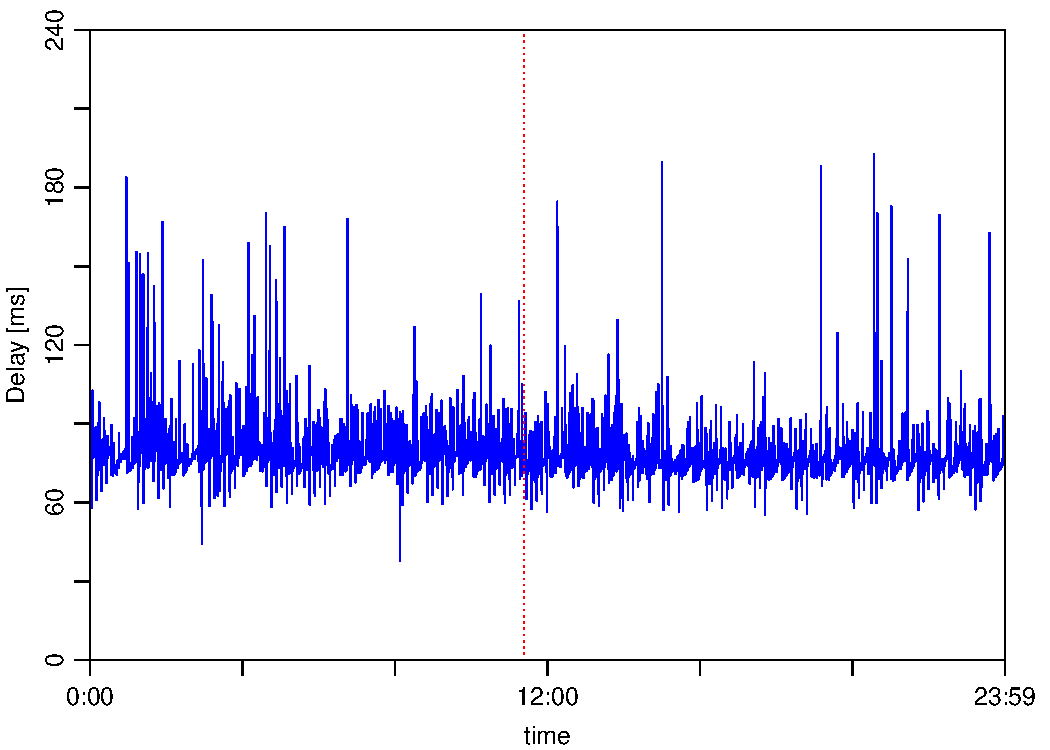
\includegraphics[width=0.5\hsize]{C:/master/mstudy/analysis/long/plot-6-26.pdf}
}~
\subfigure[6 月 27 日(土)]{
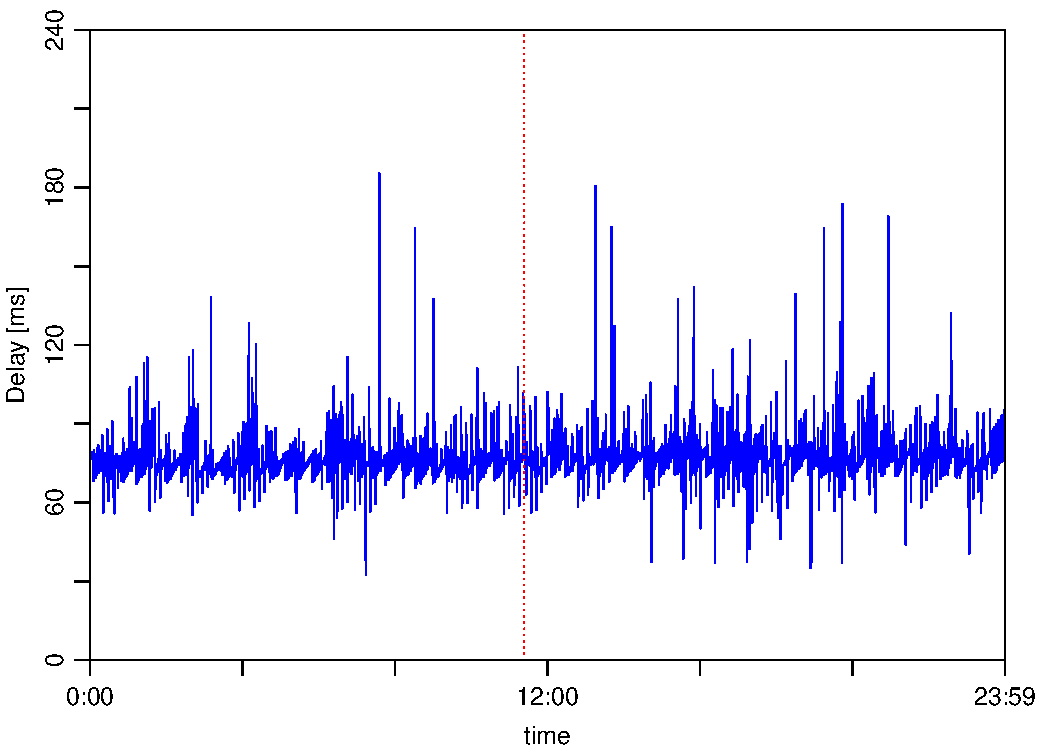
\includegraphics[width=0.5\hsize]{C:/master/mstudy/analysis/long/plot-6-27.pdf}
}
\caption{応答遅延の時間データ}
\label{otherrise}
\end{center}
\end{figure}

産業用モニタリングシステムにおける障害検知手法の開発に向けて,通常とは異なる遅延変動を通常時のものと切り分け検知するために,通常時の応答遅延の時間データをモデル化することに取り組んだ.
モデル化することで例えば,実環境でリアルタイムに得られる計測値とモデルでの予測値を逐次比較して検知したり,モデルパラメータを計測日時特有もしくは共通した特徴量とみなし,実環境でリアルタイムに計測データのモデル化を行いこの特徴量を比較して検知したりする手法が可能ではないかと考えた.

\section{目的}
モデル化に向けて計測データの波形から右肩上がりの傾向を示す区間の両端の時刻を抽出し,これら区間の時間的長さの分布や相関関係の有無を得ることを目的とする.

\section{計測データの前処理}
計測データは図 \ref{rise} のように短期的な変動が激しく特に突発的に特出して大きなまたは小さな応答遅延が発生するため,こののこぎり型の波形の抽出が困難である.
そこで計測データに対してローパスフィルタを用いて短期的な変動を生じさせる高周波数帯を除去し,逆フーリエ変換を行い復元した波形からのこぎり波の抽出を行う.

6 月 23 日の計測データに対してこの前処理をローパスフィルタの値を変えながら施し,それぞれに対して計測時刻が 0 時から 6 時までの一部の波形を図 \ref{lowpass} に示す.
ただし,横軸は計測時刻が早いものから順に 0,1,$\ldots$ としたインデックスを取り,縦軸には応答遅延の値を取っている.
また,青色線が計測値を,赤色線が前処理後の波形を表す.
\begin{figure}[tb]
\begin{center}
\subfigure[$\alpha=0.005$]{
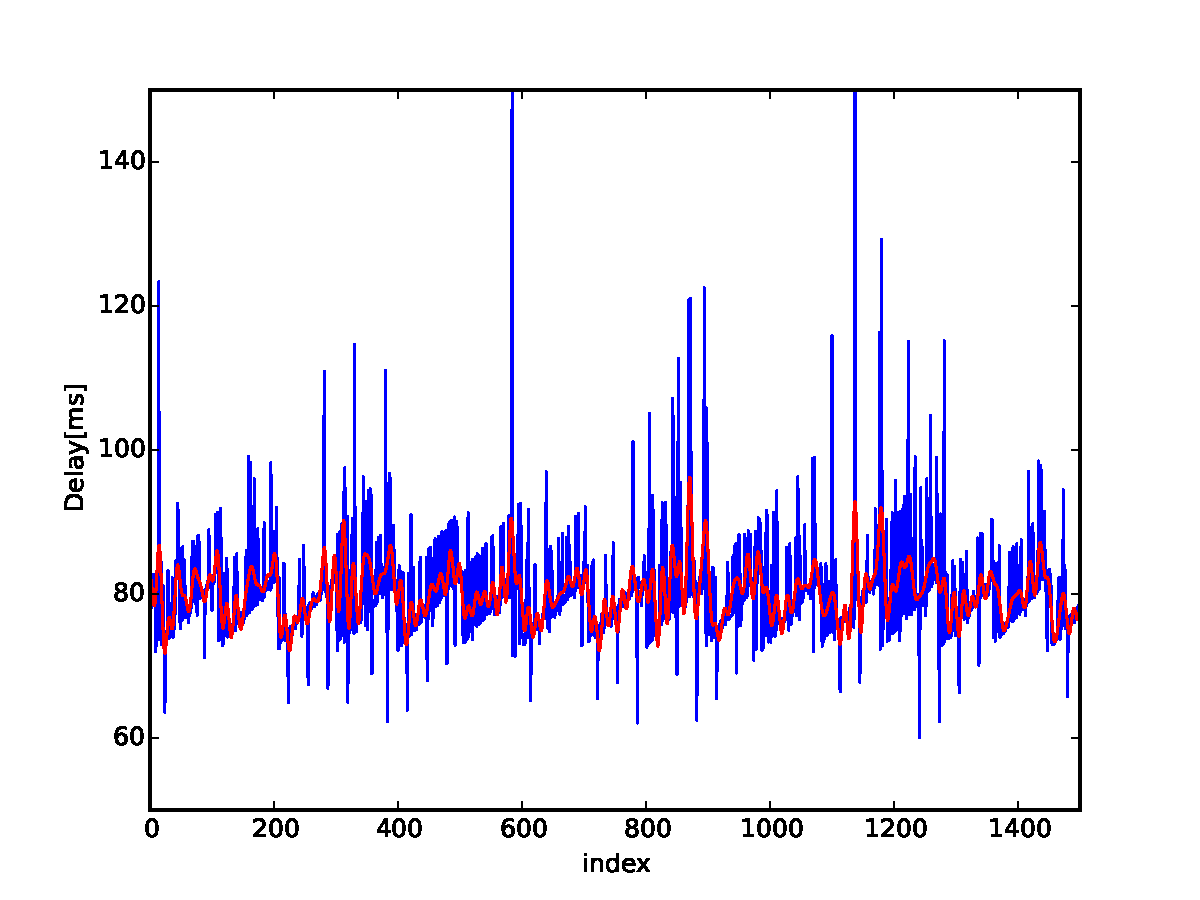
\includegraphics[width=0.5\hsize]{C:/master/mstudy/analysis/0829/lowpass05.pdf}
}~
\subfigure[$\alpha=0.006$]{
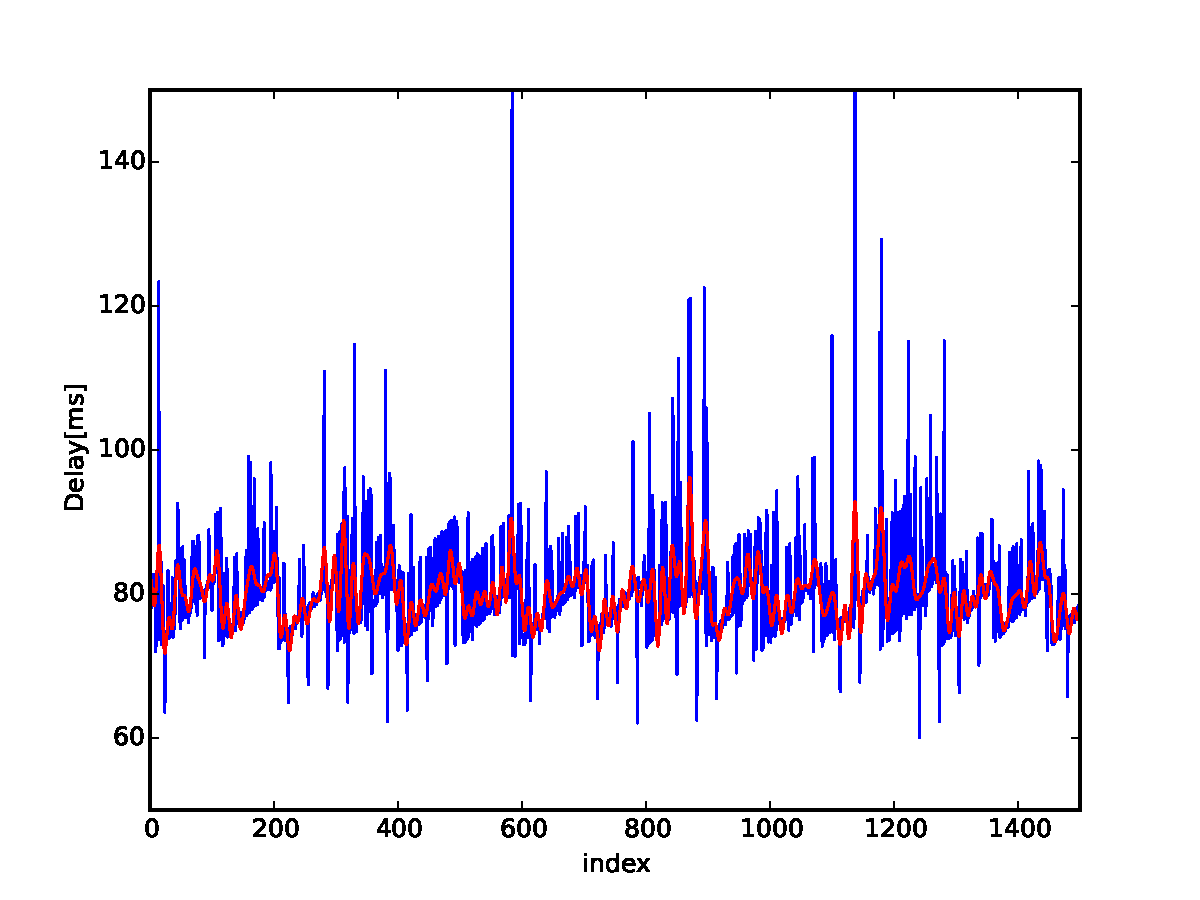
\includegraphics[width=0.5\hsize]{C:/master/mstudy/analysis/0829/lowpass06.pdf}
}\\
\subfigure[$\alpha=0.007$]{
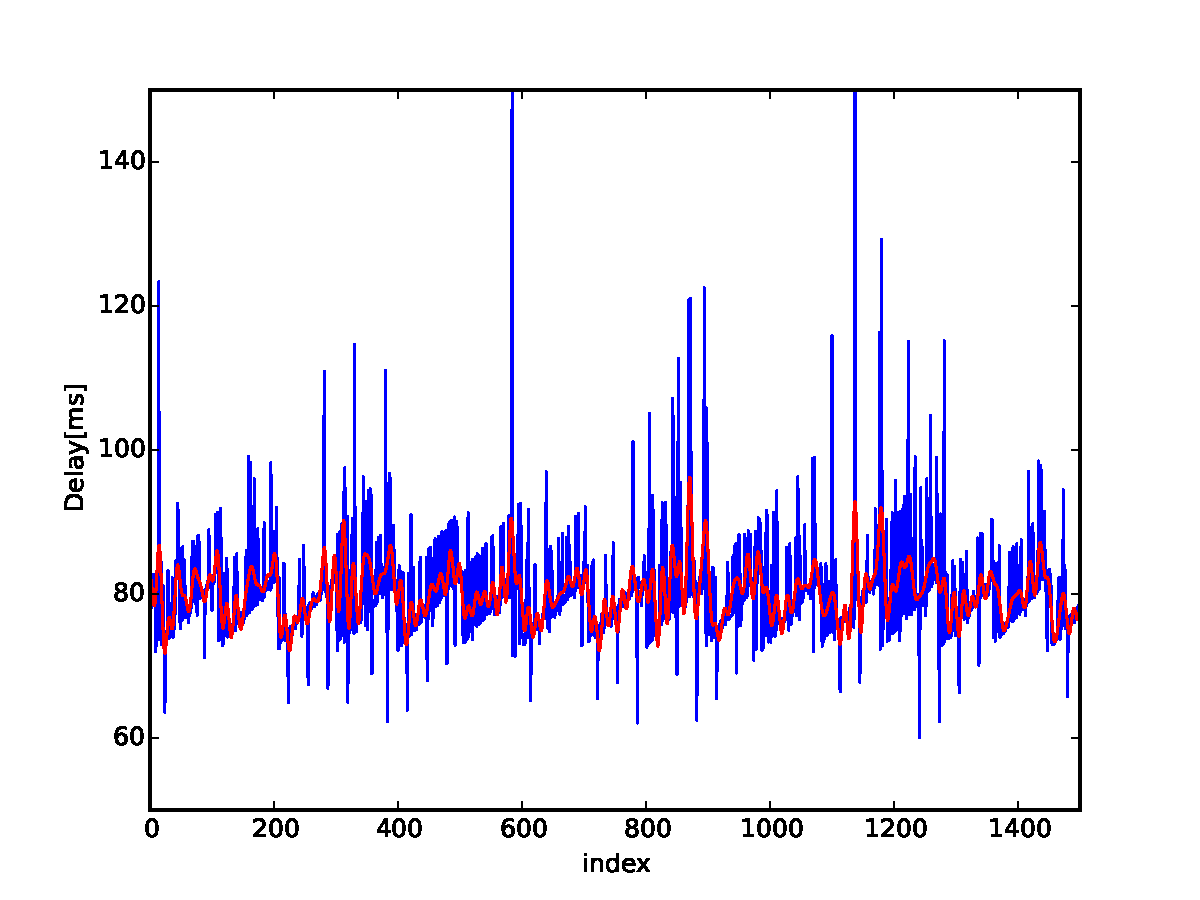
\includegraphics[width=0.5\hsize]{C:/master/mstudy/analysis/0829/lowpass07.pdf}
}~
\subfigure[$\alpha=0.008$]{
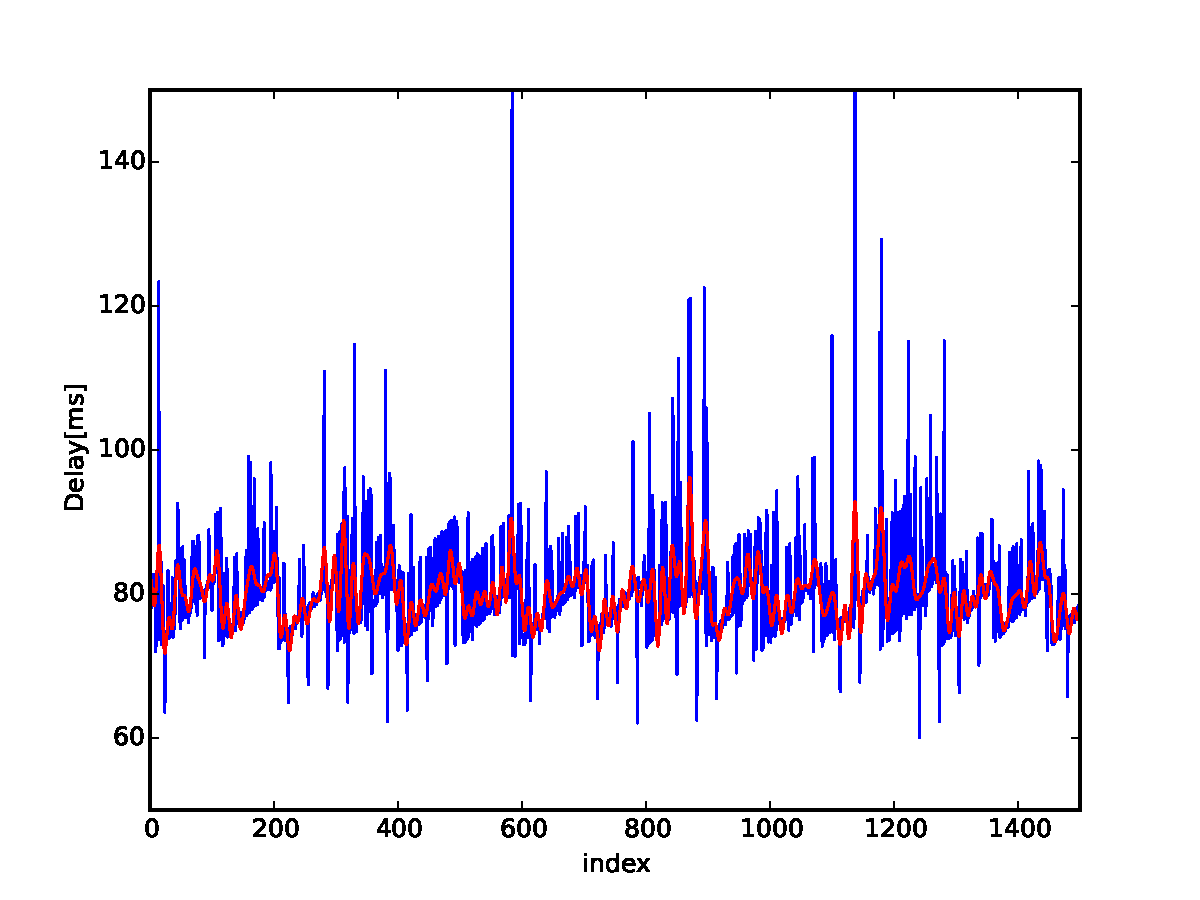
\includegraphics[width=0.5\hsize]{C:/master/mstudy/analysis/0829/lowpass08.pdf}
}\\
\subfigure[$\alpha=0.009$]{
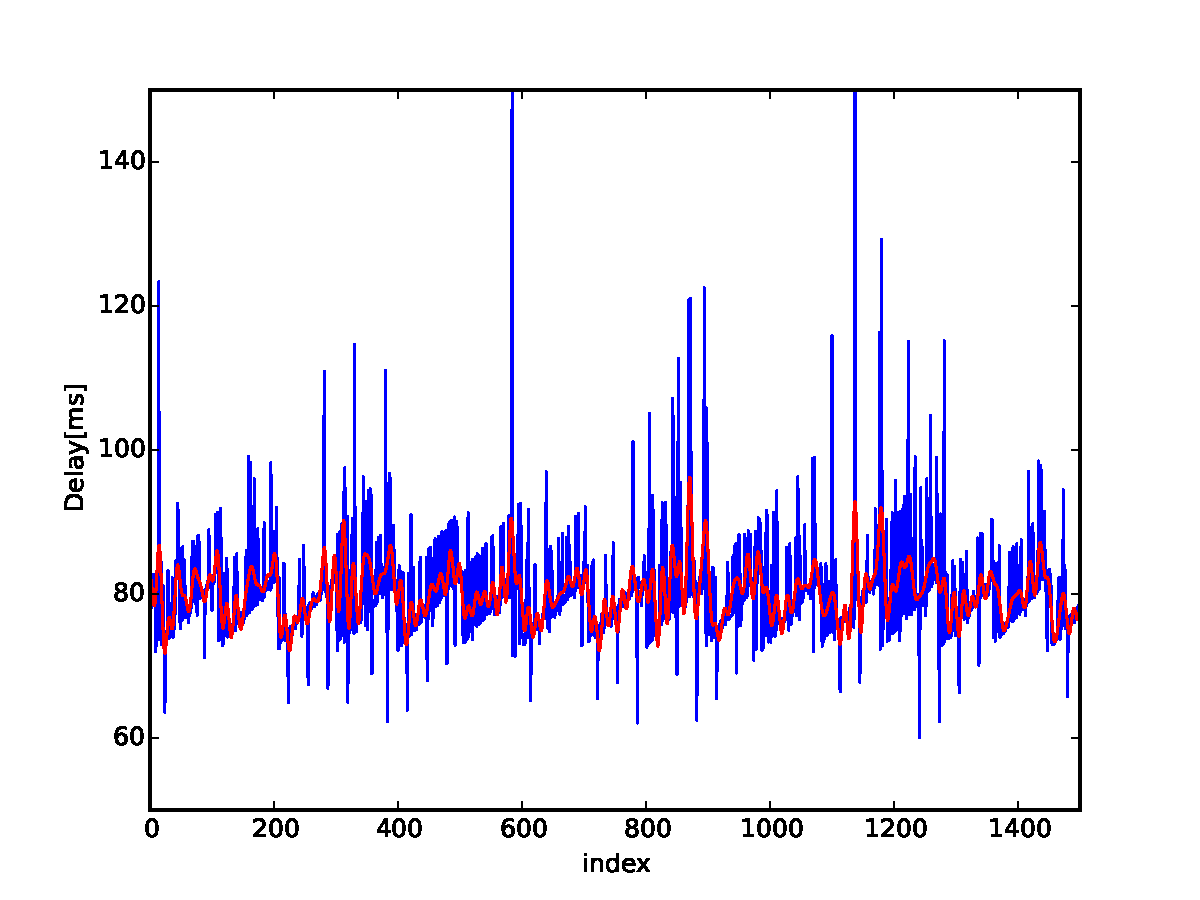
\includegraphics[width=0.5\hsize]{C:/master/mstudy/analysis/0829/lowpass09.pdf}
}~
\subfigure[$\alpha=0.010$]{
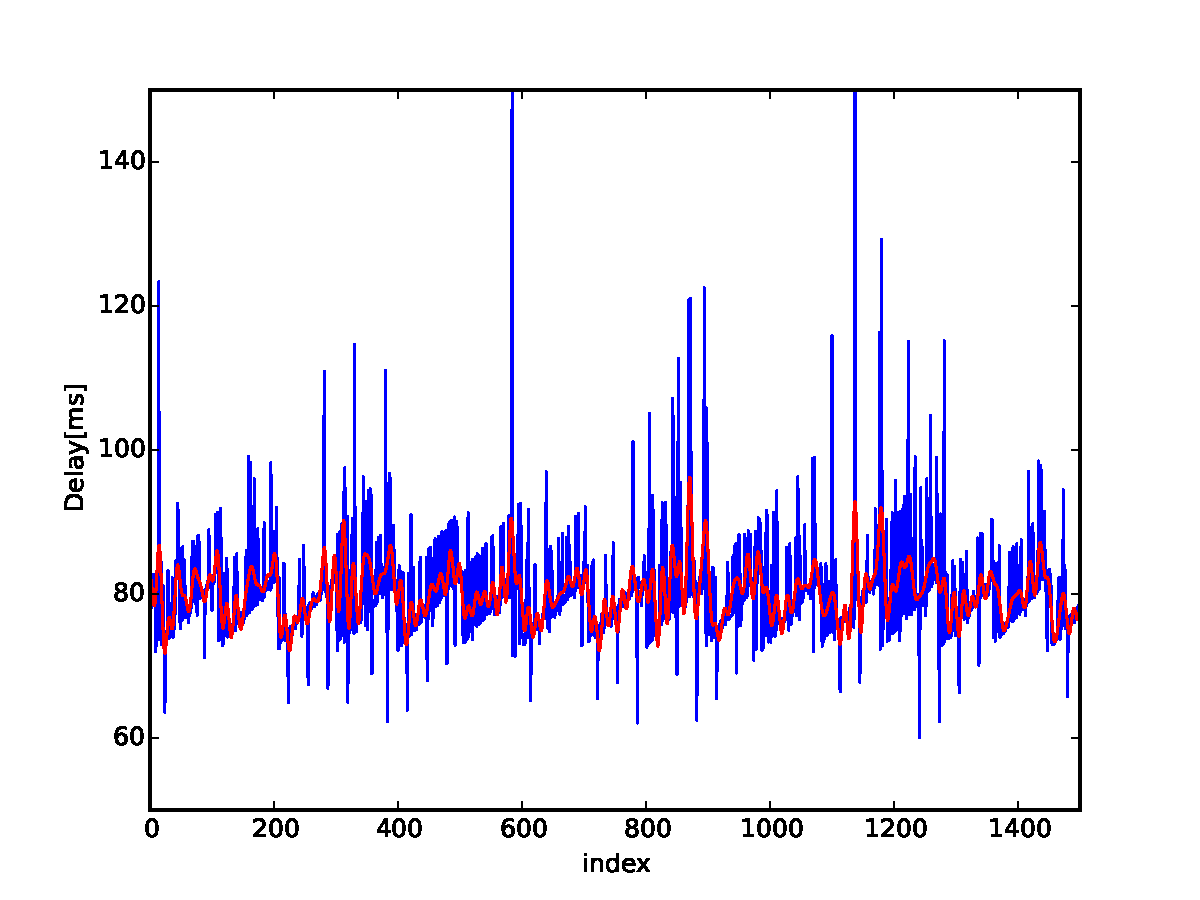
\includegraphics[width=0.5\hsize]{C:/master/mstudy/analysis/0829/lowpass10.pdf}
}\\
\caption{計測波形(青線)から $\alpha$ Hz 以上の波を除去した波形(赤線)}
\label{lowpass}
\end{center}
\end{figure}
ローパスフィルタの値はもと波形の突発的な応答遅延を除去し,かつのこぎり型の波形の各両端が滑らかになりすぎないようになるものが好ましい.
計測波形から定量的にこの値を決めることが望ましいが,ここでは図 \ref{lowpass} の結果からこの値を 0.008 Hz として話を進めることとする.

\section{手法}
図 \ref{lowpass}(d) の波形からのこぎり型の波形を抽出する方法はいくつか考えられる.
ここでは,その一つ一つを検証する.

\subsection{手法 1 : 逐次的な単回帰}
のこぎり波は右肩上がりの直線に見えるので,前処理後の波形に含まれる各のこぎり波は直線で回帰することができ,その回帰結果からのこぎり波を抽出できないかを検討した.

\subsubsection{アルゴリズム}
波形を右肩上がりの直線で回帰できる区間に分割する.
しかし,全区間を一度に分割することは分割数が未知であるため困難である.
そこで,先頭からインデックス幅 200 (計測時間 50 分相当)に含まれる波形を二つに分割したとき前後それぞれの波形を最も精度良く右肩上がりの直線で回帰できる分割点を求め,次はその分割点からさらにインデックス幅 200 までの波形に対して同様の操作により分割点を求める.
この操作を繰り返すことで全体を分割する.
また,このインデックス幅 200 は計測時間 50 分相当であり,6 月 23 日の全区間の計測データに対して FFT を行った結果である図 \ref{fft} からのこぎり型の波形の周期が大体 25 分程度(約 0.0006 Hz)であることをもとに,のこぎり型波形が 2 つよりも多く含まれないように定めた.
\begin{figure}[tb]
\begin{center}
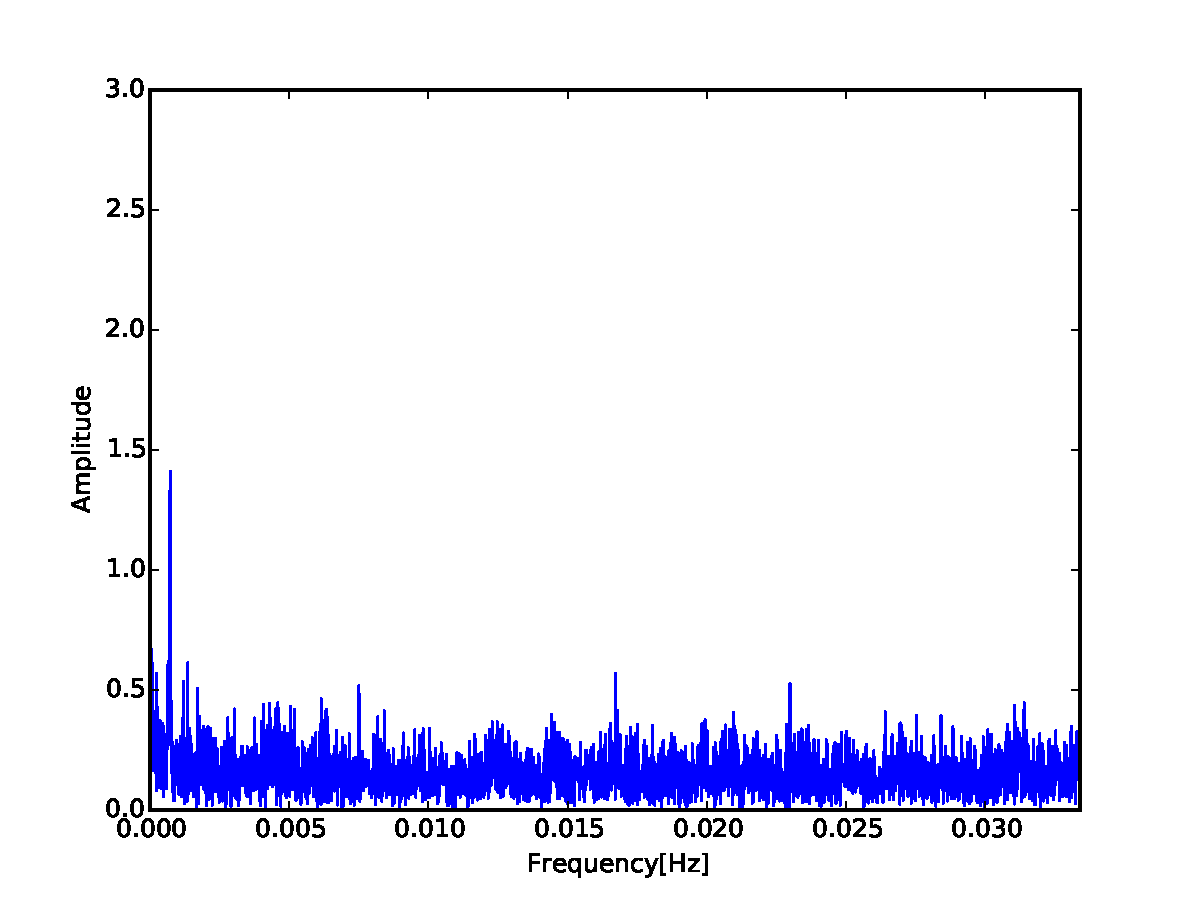
\includegraphics[width=0.65\hsize]{C:/master/mstudy/analysis/0829/fft_6-23.pdf}
\caption{6 月 23 (火)の全区間データに対する FFT (横軸 : 周波数,縦軸 : 振幅)}
\label{fft}
\end{center}
\end{figure}

単回帰には最小二乗法を用い,回帰精度の指標として決定係数の積を用いた.
分割点はインデックス幅 200 の区間で前後二つの回帰線の傾きが共に正かつ指標の値を最大とする時点とする.
また,各回帰線は少なくとも 20 点(約 5 分相当)以上の計測点を回帰するものとする.
表 \ref{alg1} にこの分割方法の疑似コードを示す.\\
\begin{table}[tb]
\caption{逐次的単回帰のアルゴリズム}
\label{alg1}
\begin{tabular}{l}
\hline
$Data$ = (前処理後のデータ列)\\
$C$ = [0] \hspace{1cm}\#分割点のリスト\\
\\
while(1)\{\\
\hspace{0.5cm}for ($20 \leq i \leq 180$)\{\\
\hspace{1cm}$left = C[末尾]$\\
\hspace{1cm}$mid = C[末尾] + i$\\
\hspace{1cm}$right = C[末尾] + 200$\\
\\
\hspace{1cm}$X_1 = 区間 [left, mid)$\\
\hspace{1cm}$Y_1 = Data[X_1]$\\
\\
\hspace{1cm}$X_2 = 区間 [mid, right]$\\
\hspace{1cm}$Y_2 = Data[X_2]$\\
\\
\hspace{1cm}$\widehat{Y_1} = a_1\widehat{X_1} + b_1 \leftarrow 最小二乗法(X_1,Y_1)$\\
\hspace{1cm}$\widehat{Y_2} = a_2\widehat{X_2} + b_2 \leftarrow 最小二乗法(X_2,Y_2)$\\
\hspace{0.5cm}\}\\
\\
\hspace{0.5cm}if($a_1>0$ and $a_2>0$)\\
\hspace{1cm}$C = C \cup \argmax_{20\leq mid \leq 180} \left[1-\frac{\sum \left(Y_1 - \widehat{Y_1}\right)^2}{\sum \left(Y_1 - \overline{Y_1}\right)^2} \right] * \left[1-\frac{\sum \left(Y_2 - \widehat{Y_2}\right)^2}{\sum \left(Y_2 - \overline{Y_2}\right)^2} \right]$\hspace{1cm}$\#\overline{Y}$ は $Y$ の平均値\\
\\
\hspace{0.5cm}if($mid + 200 > データ数)$\hspace{1cm}break\\
\}
\end{tabular}
\end{table}

\subsubsection{実行結果}
実行結果を図 \ref{resultalg1} に示す.
この図は黒線が前処理後の波形を示しており,色線は分割点で分割された各区間の波形の回帰直線である.
これらはともに図の左側を縦軸としている.
また,右側の縦軸には評価値を取っており,アルゴリズム実行中において各色の回帰直線の終了時点に当たる分割点を求める際の評価値を回帰直線と同色の曲線で示した.
\begin{figure}[tb]
\begin{center}
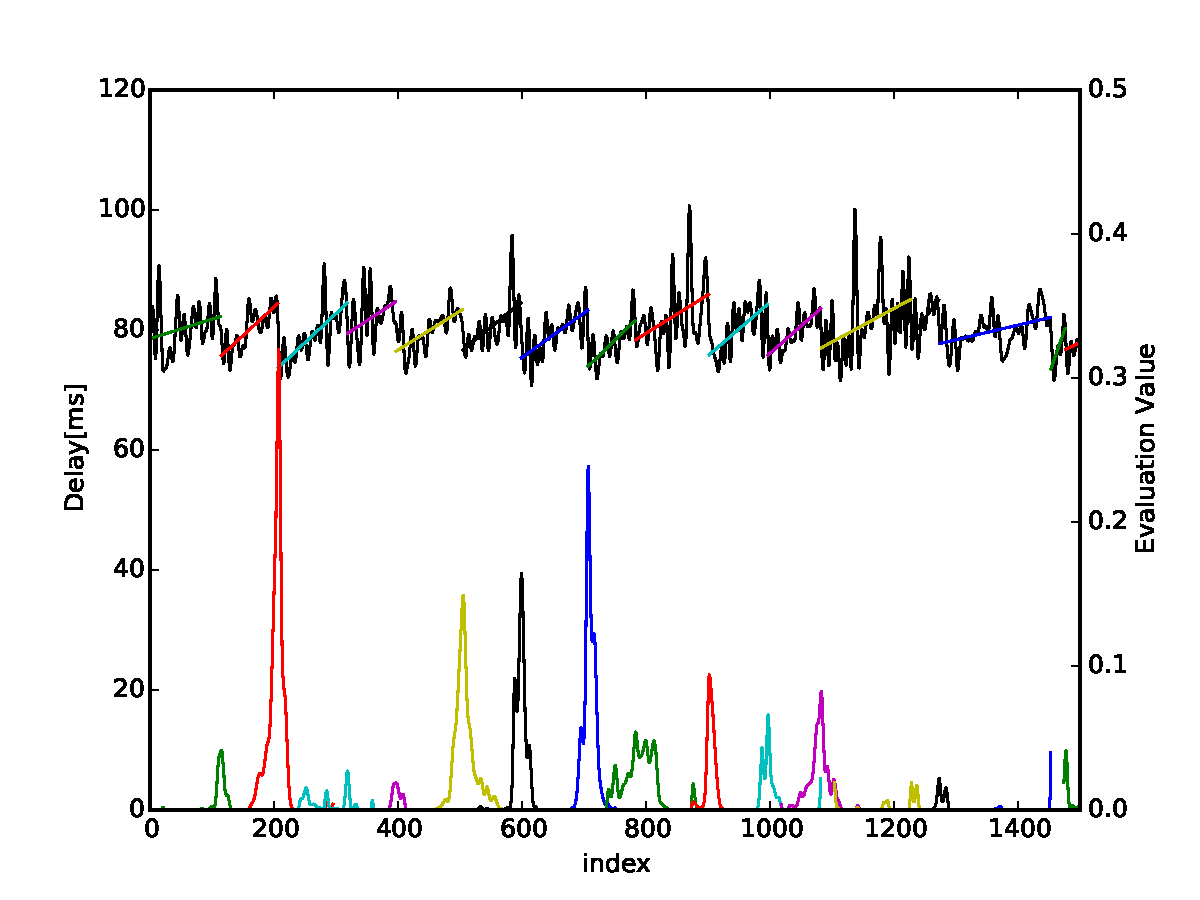
\includegraphics[width=\hsize]{C:/master/mstudy/analysis/0829/resultalg1.pdf}
\caption{手法 1 の実行結果と評価値}
\label{resultalg1}
\end{center}
\end{figure}

図より,おおよそ期待通りの分割がなされており,またこの評価値による分割点の感度は高いことが見て取れる.しかしながら一方で,インデックス 1300 から 1400 の区間では 1350 付近での分割が期待されるがなされていない.これは,最小二乗法による単回帰では回帰線と計測値の誤差を小さくするが,回帰線と計測値の大小関係は考慮していないことから,のこぎり波の両端を示す急激な下振れを検出できなかったと考えられる.
また,インデックス 1100 から 1300 までの区間のように評価値に明確な極大値が存在しないこともあるようだ.

\subsection{手法 2 : 累積積分}
のこぎり波の分割点直前の波形は直後のものに比べて大きな値をとっている.
したがって,前処理後の波形のインデックス 0 からの累積積分値は分割点前で傾きが増加していき,直後では傾きが減少すると考えられる.
つまり,分割点は累積積分関数の傾きの変化率が正から負に切り替わる変曲点であると考えられる.
そこでここでは,累積積分関数の変曲点を分割点として抽出できないかを検討した.

\subsubsection{アルゴリズム}
前処理後の計測波形は 15 秒毎の離散データである.
この離散データを $x_i (i = 0,1,\ldots)$と表したとき,累積積分関数 $I_n$ とその微分は以下のように定まる.
$$I_n = \sum_{i=0}^n x_i$$
$$I_n^{\prime} = \frac{1}{2}(I_{n+1} - I_{n-1})$$
この時,変曲点 $i$ は $I_i^{\prime \prime} \geq 0$ かつ $I_{i+1}^{\prime \prime} \leq 0$ で求められる.
また,前処理後の波形において分割点直前のある程度の区間の波は直後のある程度の区間の波に比べて大きくなることを考慮し,分割点は変曲点 $i$ のうち,パラメータ $l$ と $\alpha$ を用いて以下の式を満たすものとする.
$$\frac{\sum_{j = i}^{i+l-1} x_j}{\sum_{j = i-l}^{i-1} x_j} \leq \alpha$$

\subsubsection{実行結果}
パラメータ $l$ と $\alpha$ を変えながら行った実行結果を図 \ref{resultalg2-1} から図 \ref{resultalg2-2} に示す.
これらの図は黒線が前処理後の波形を示しており,青線は正規化した累積積分関数である.
また,赤点で黒線上に分割点を,青線上に分割点に対応する累積積分関数上の点を示した.
\begin{figure}[tb]
\begin{center}
\subfigure[$l = 5$]{
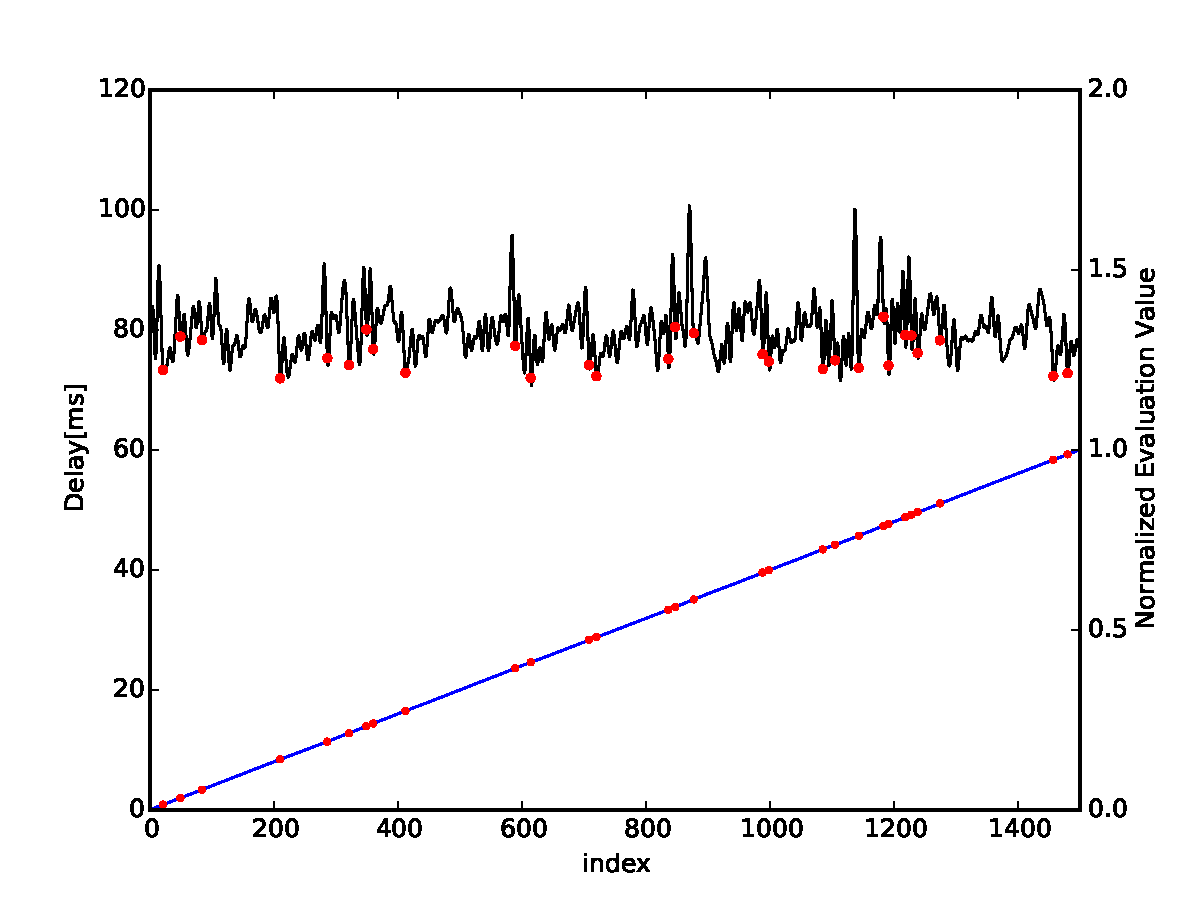
\includegraphics[width=0.5\hsize]{C:/master/mstudy/analysis/0829/result_integral_width5_alpha095.pdf}
}~
\subfigure[$l = 10$]{
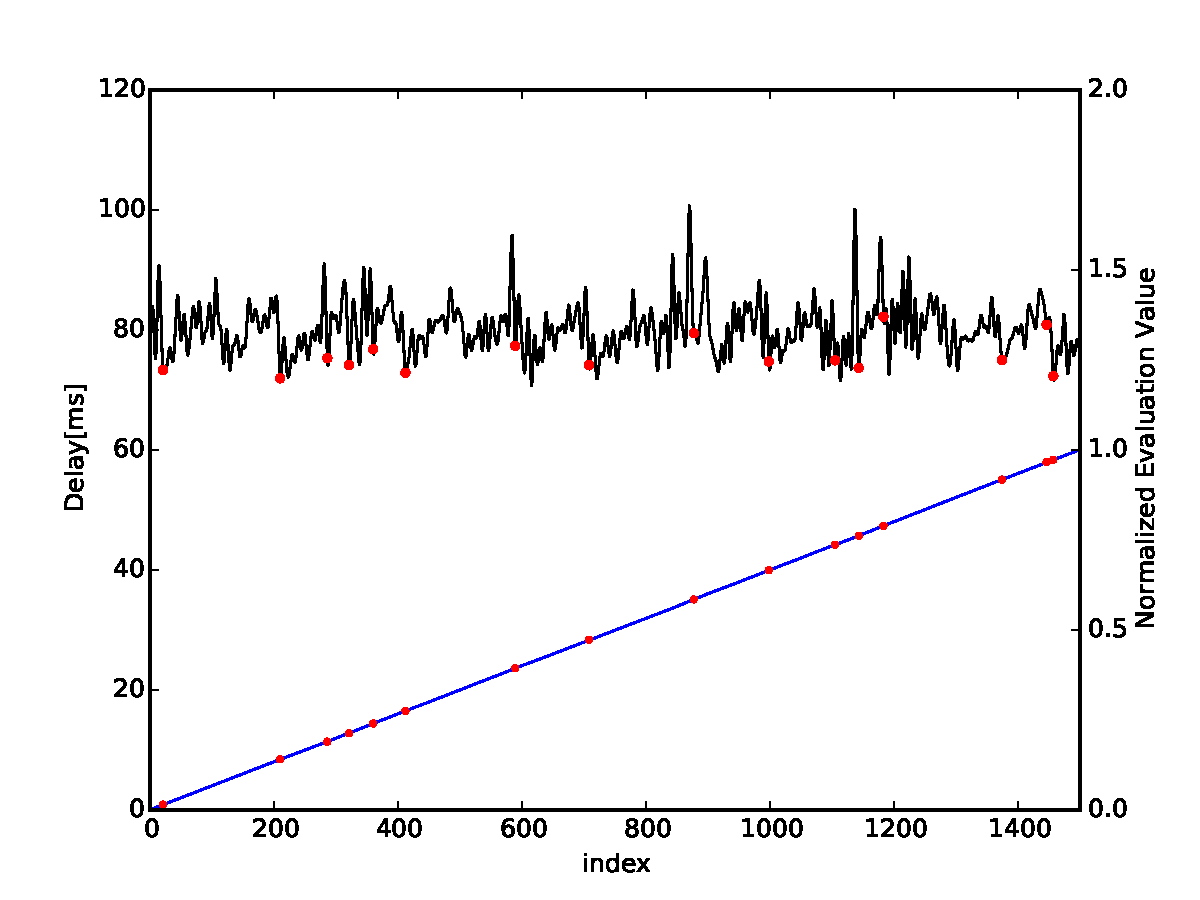
\includegraphics[width=0.5\hsize]{C:/master/mstudy/analysis/0829/result_integral_width10_alpha095.pdf}
}\\
\subfigure[$l = 15$]{
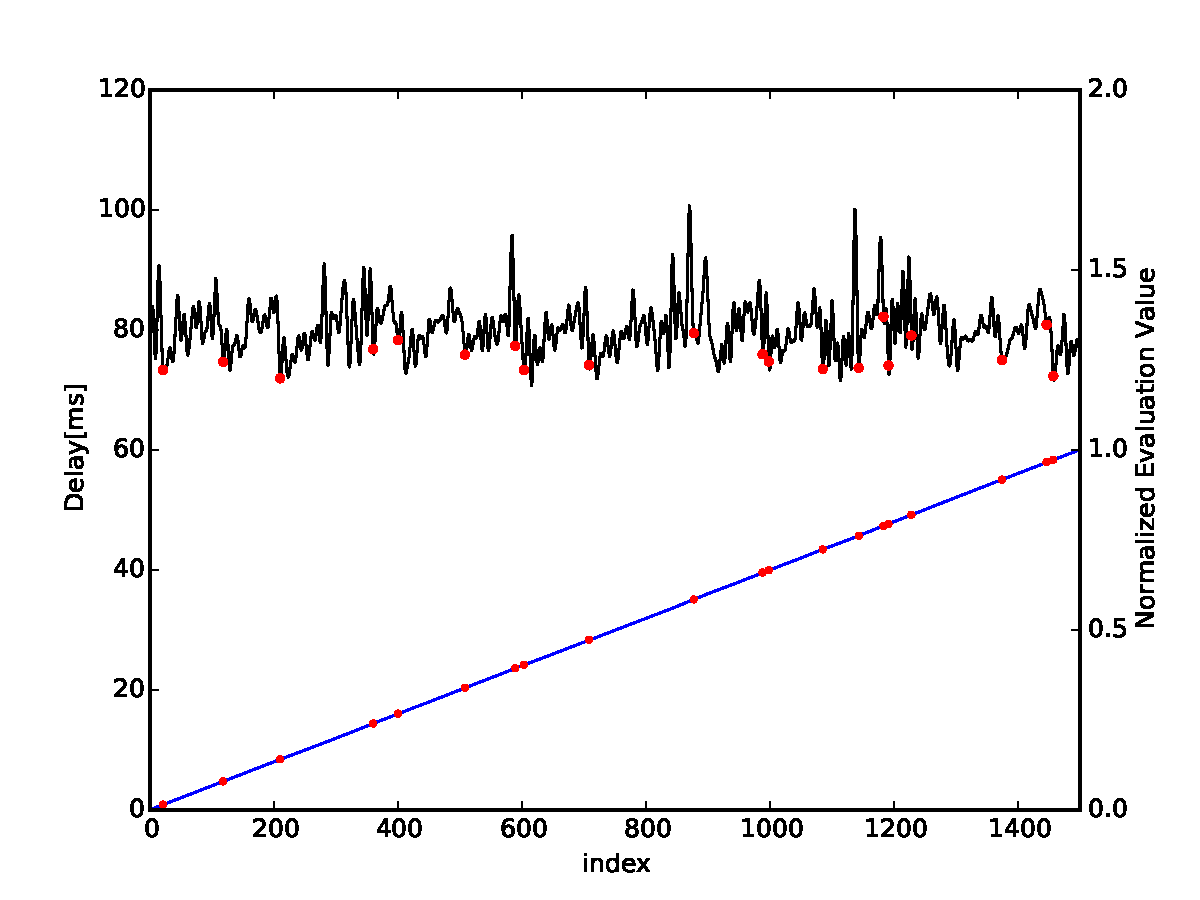
\includegraphics[width=0.5\hsize]{C:/master/mstudy/analysis/0829/result_integral_width15_alpha095.pdf}
}~
\subfigure[$l = 20$]{
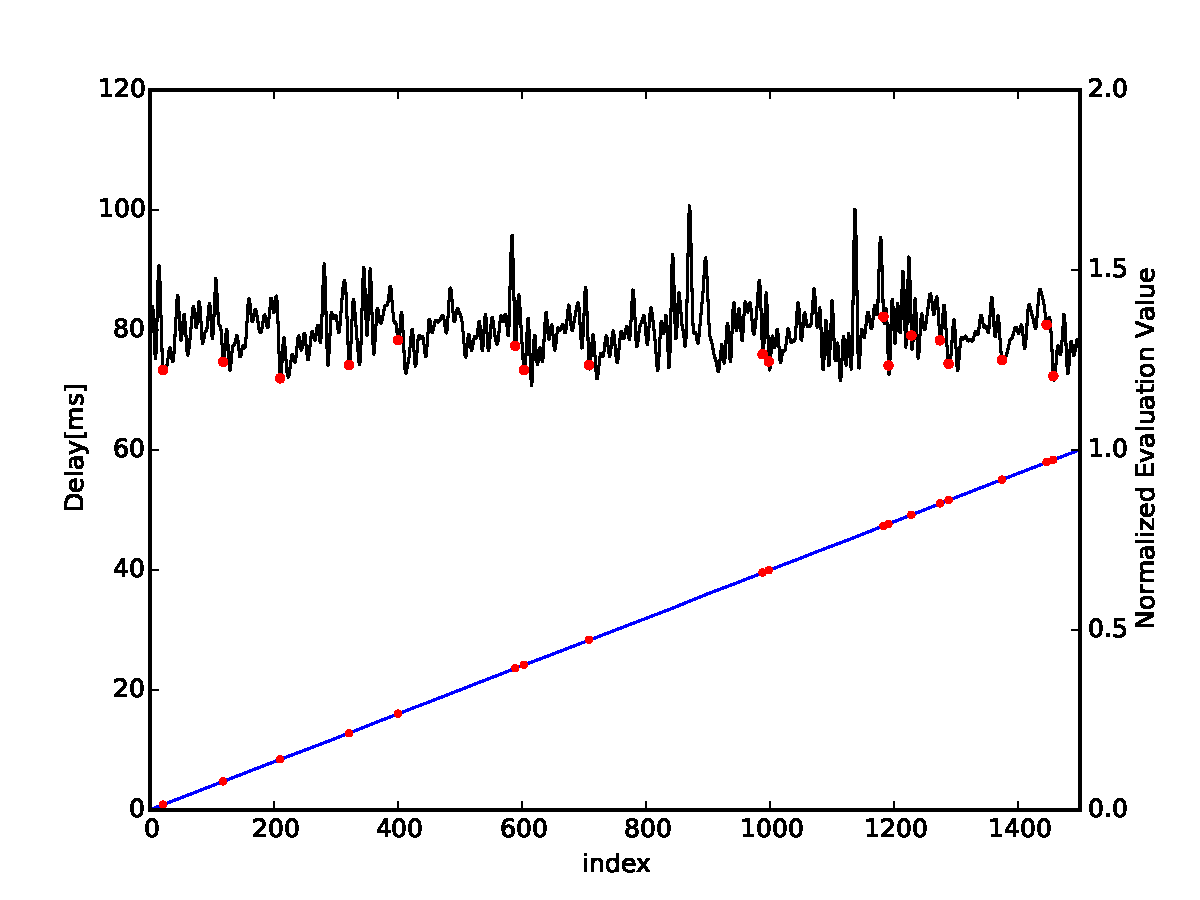
\includegraphics[width=0.5\hsize]{C:/master/mstudy/analysis/0829/result_integral_width20_alpha095.pdf}
}\\
\caption{手法 2 の実行結果($\alpha=0.95$)}
\label{resultalg2-1}
\end{center}
\end{figure}
\begin{figure}[tb]
\begin{center}
\subfigure[$l = 5$]{
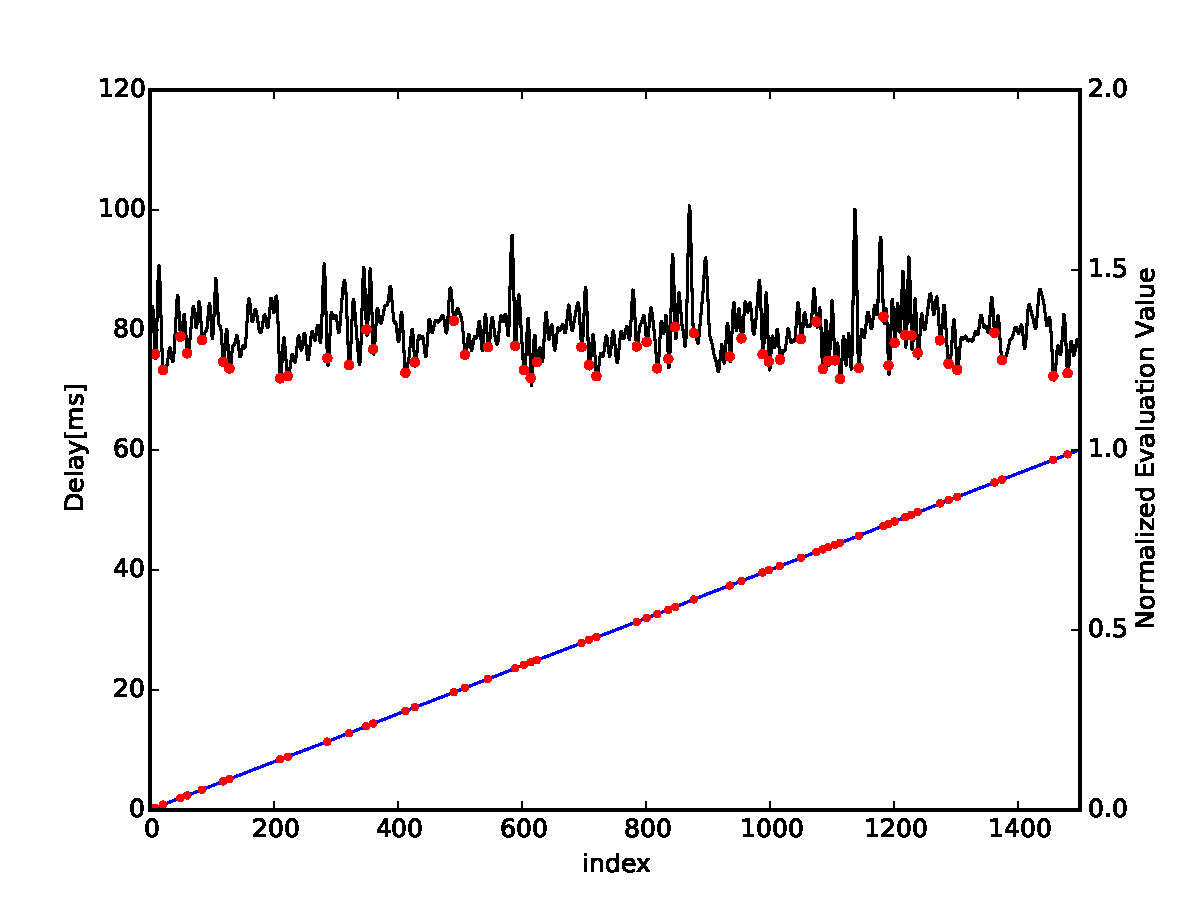
\includegraphics[width=0.5\hsize]{C:/master/mstudy/analysis/0829/result_integral_width5_alpha097.pdf}
}~
\subfigure[$l = 10$]{
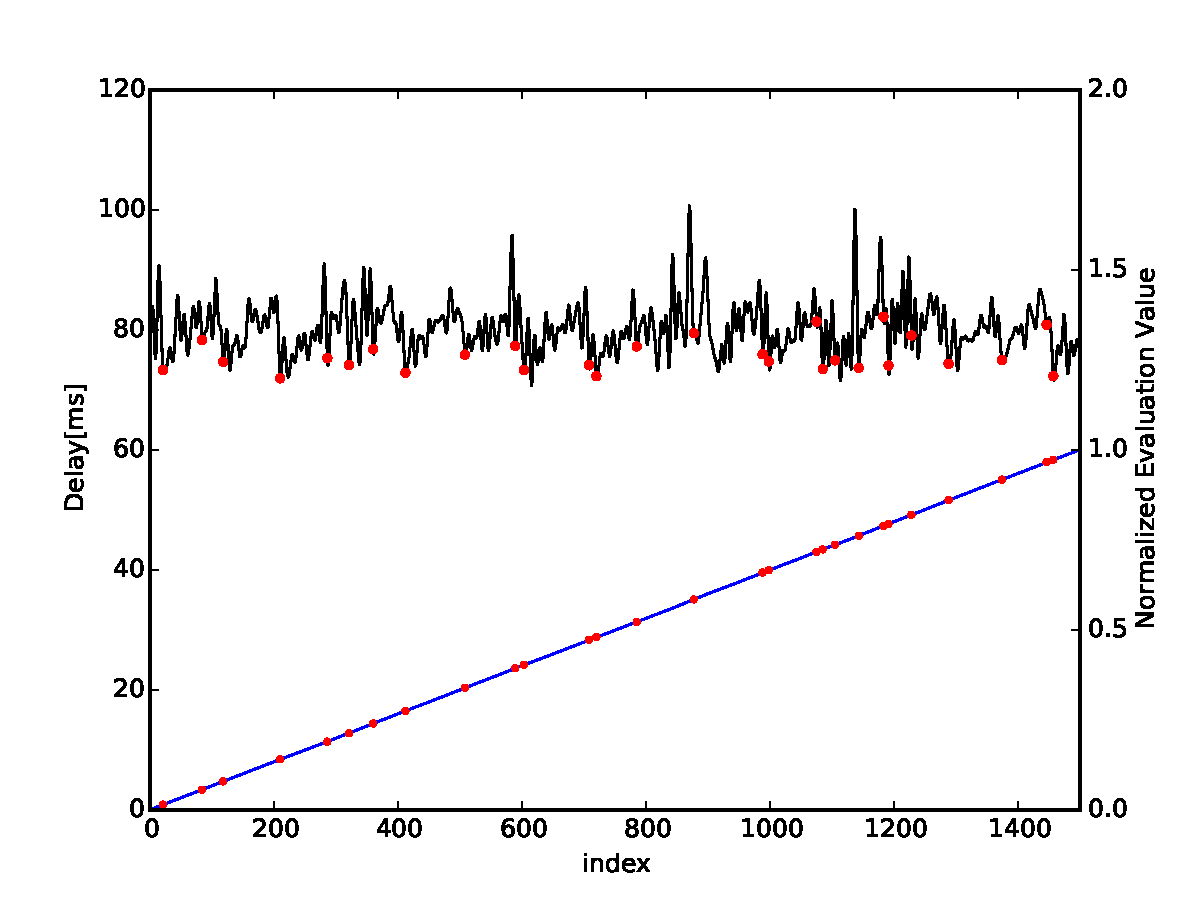
\includegraphics[width=0.5\hsize]{C:/master/mstudy/analysis/0829/result_integral_width10_alpha097.pdf}
}\\
\subfigure[$l = 15$]{
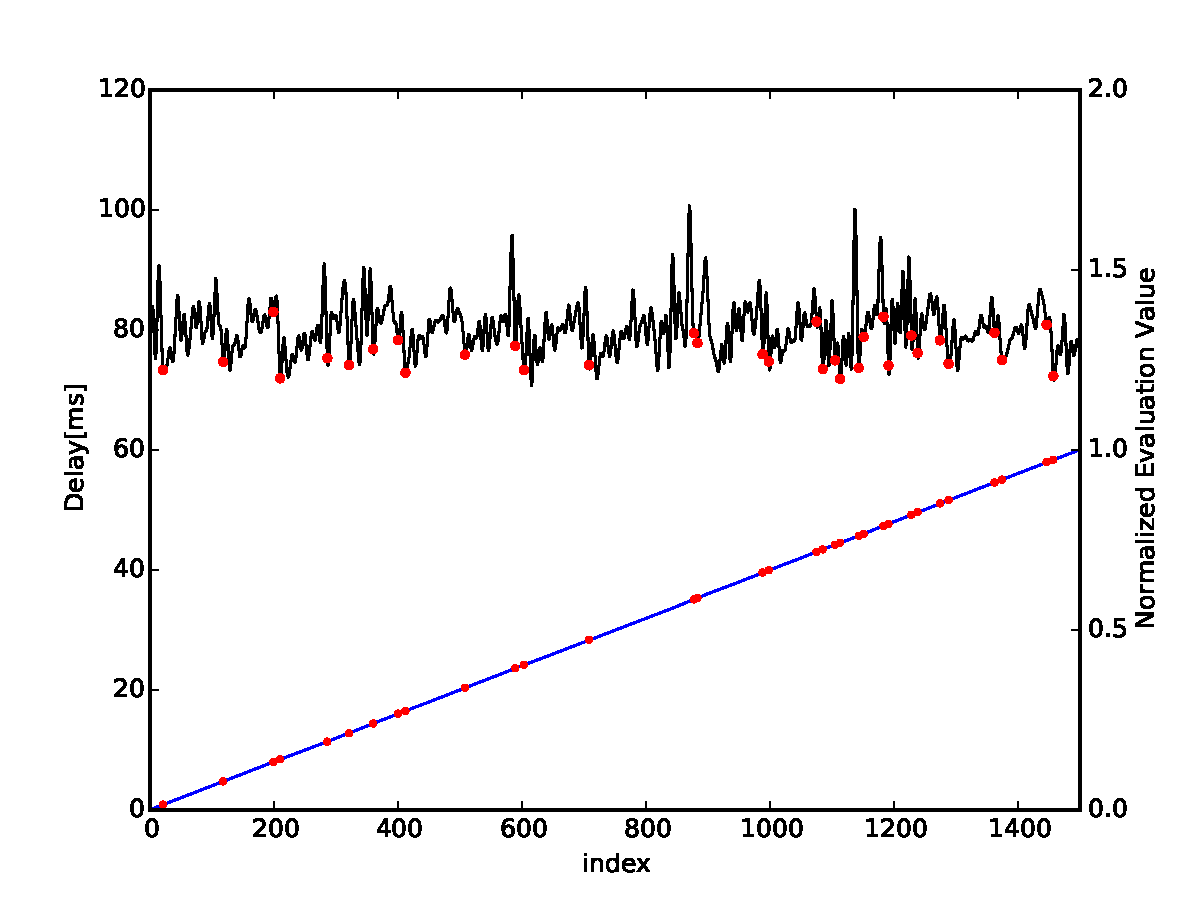
\includegraphics[width=0.5\hsize]{C:/master/mstudy/analysis/0829/result_integral_width15_alpha097.pdf}
}~
\subfigure[$l = 20$]{
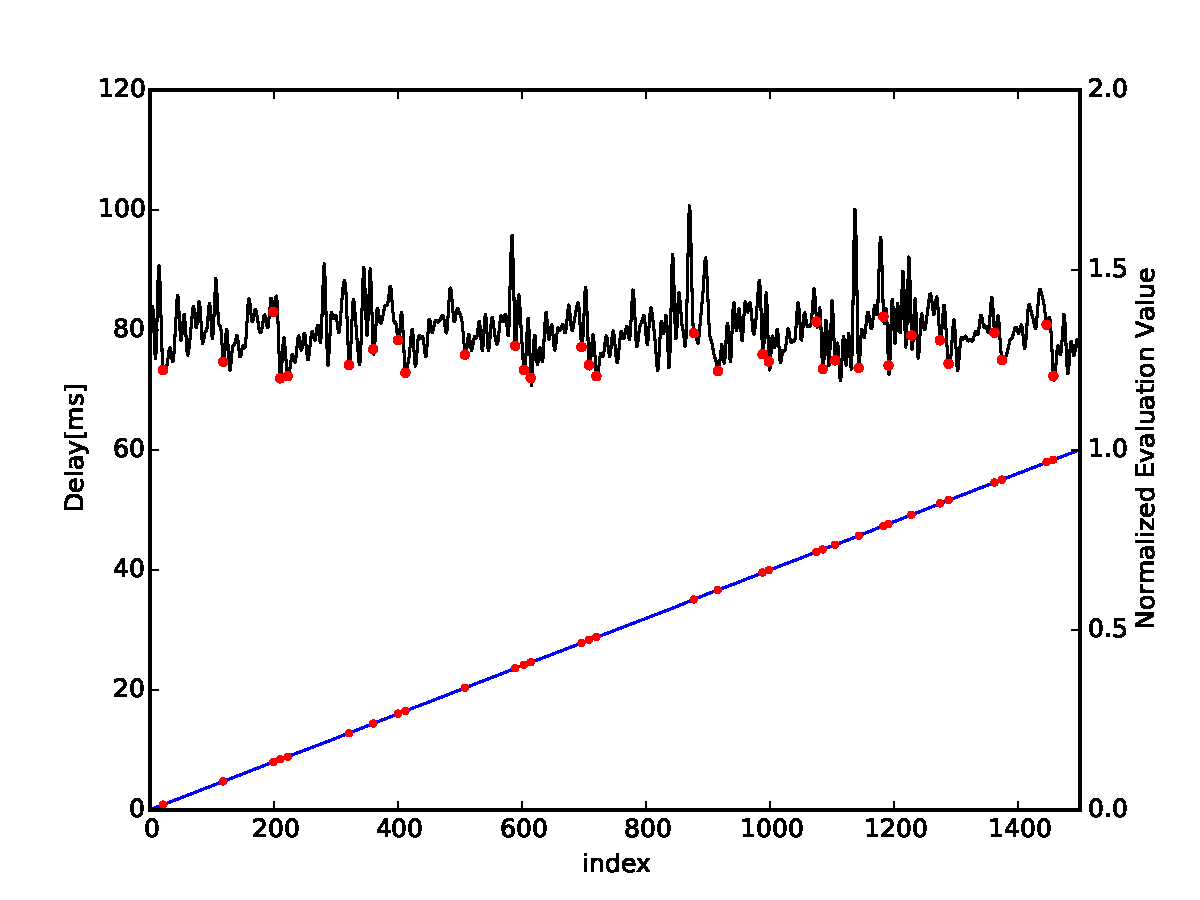
\includegraphics[width=0.5\hsize]{C:/master/mstudy/analysis/0829/result_integral_width20_alpha097.pdf}
}\\
\caption{手法 2 の実行結果($\alpha=0.97$)}
\end{center}
\end{figure}
\begin{figure}[tb]
\begin{center}
\subfigure[$l = 5$]{
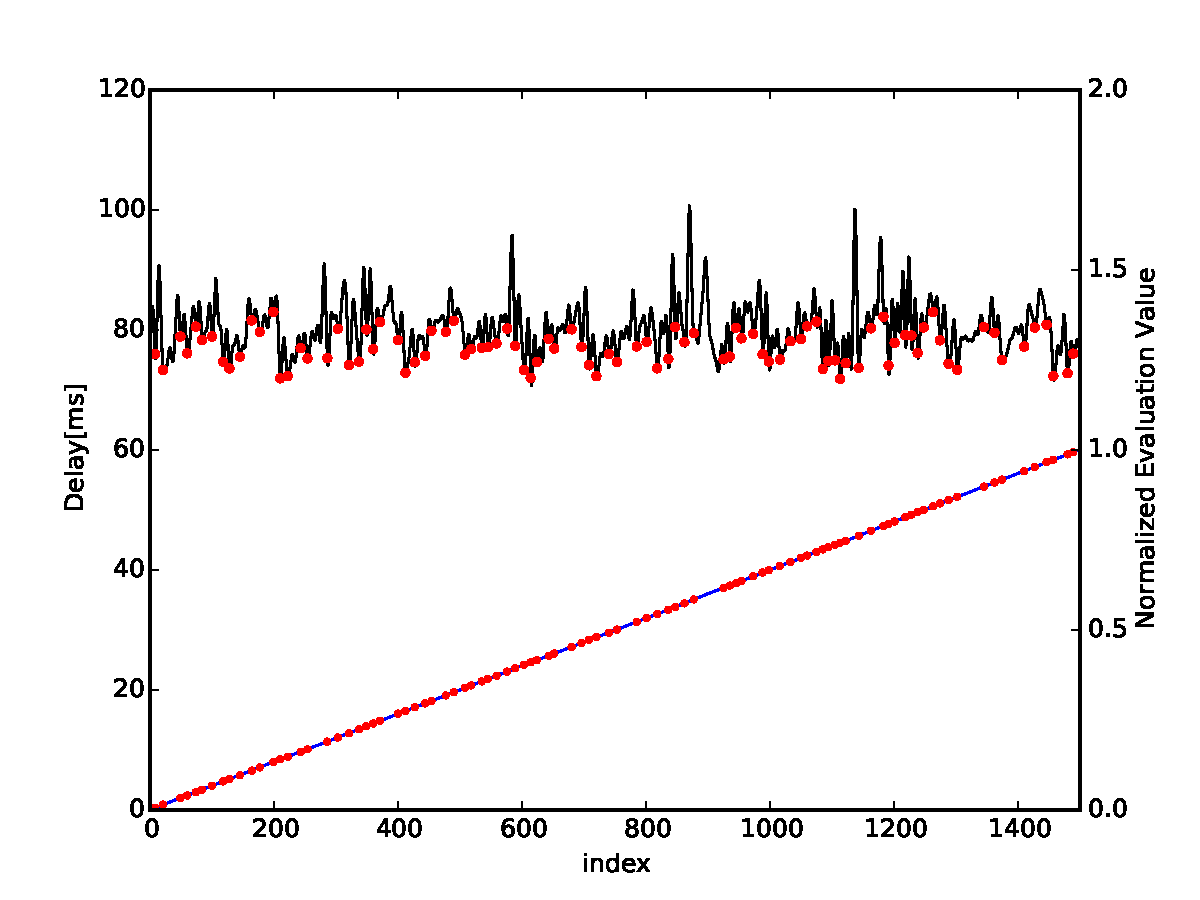
\includegraphics[width=0.5\hsize]{C:/master/mstudy/analysis/0829/result_integral_width5_alpha099.pdf}
}~
\subfigure[$l = 10$]{
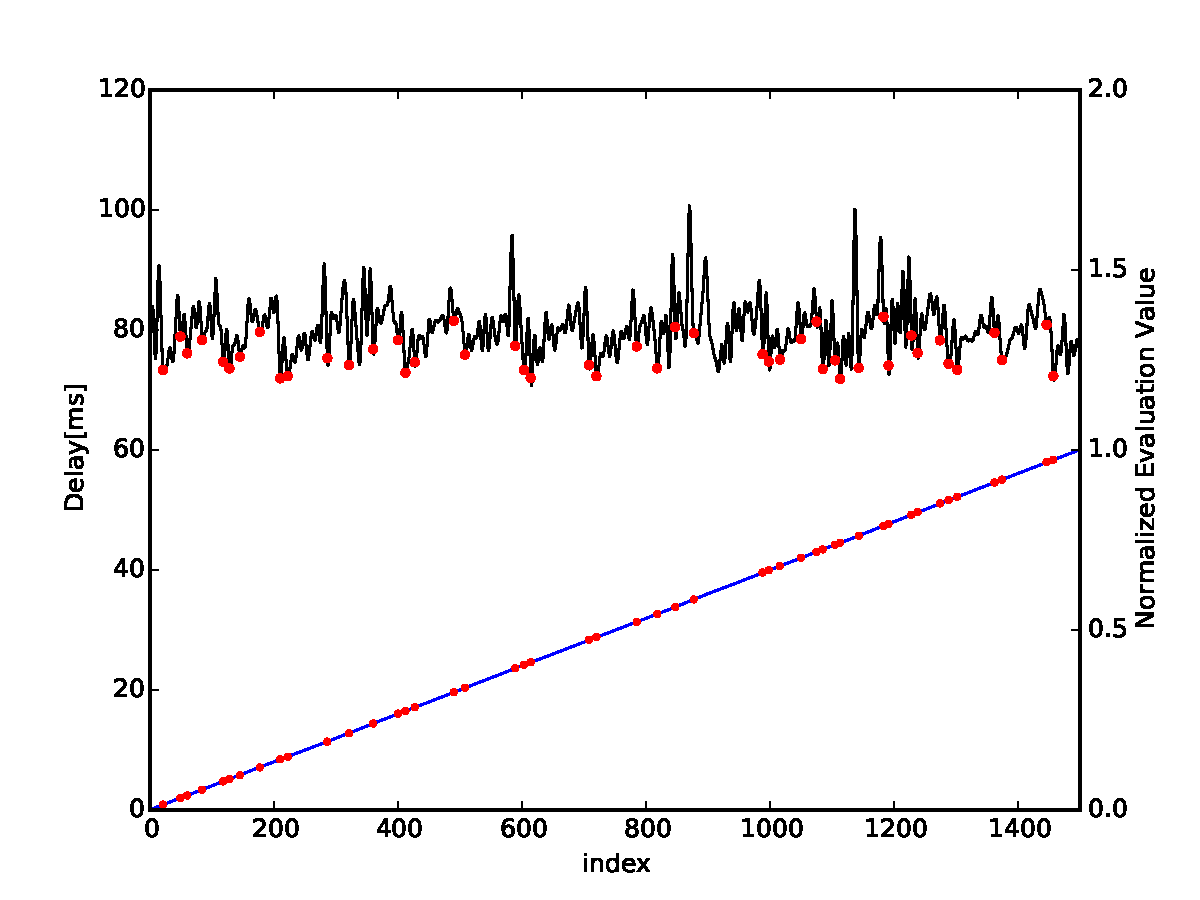
\includegraphics[width=0.5\hsize]{C:/master/mstudy/analysis/0829/result_integral_width10_alpha099.pdf}
}\\
\subfigure[$l = 15$]{
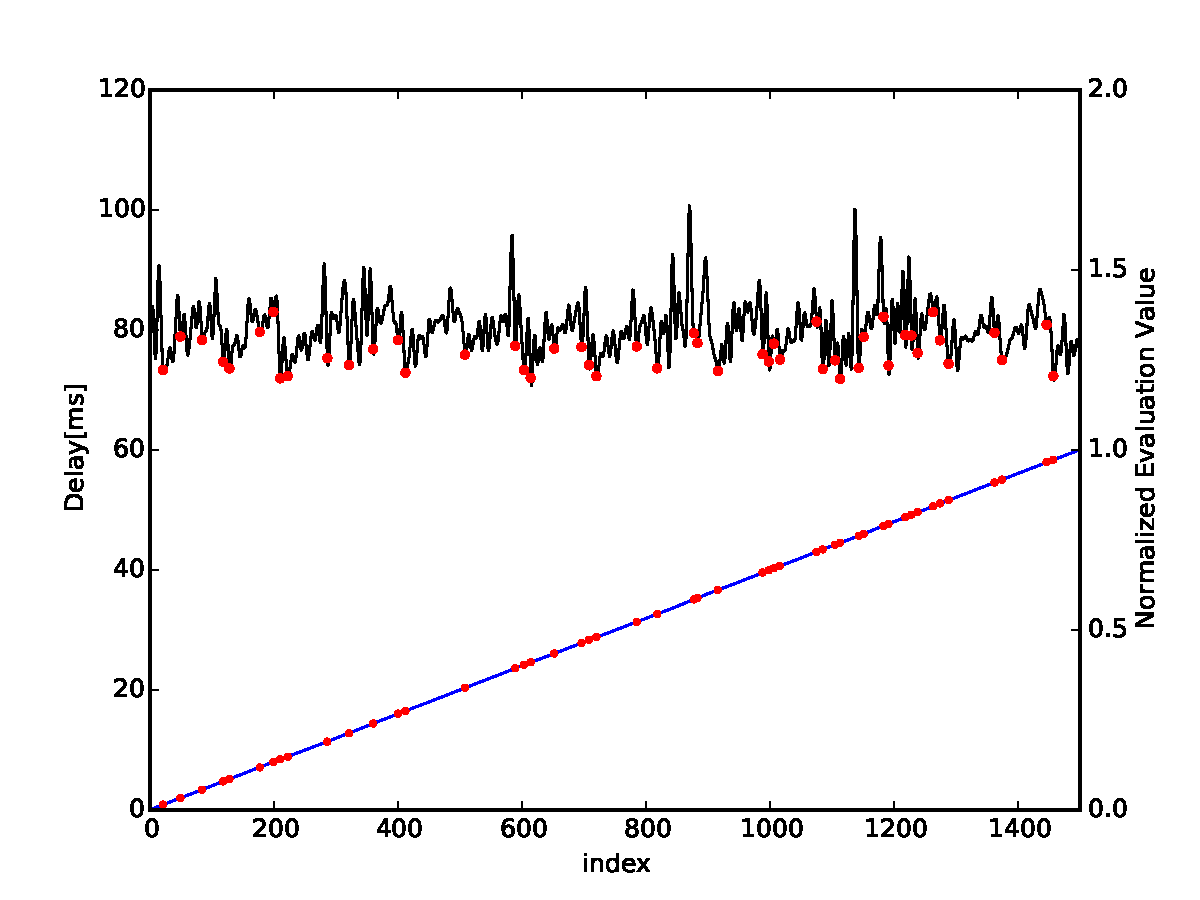
\includegraphics[width=0.5\hsize]{C:/master/mstudy/analysis/0829/result_integral_width15_alpha099.pdf}
}~
\subfigure[$l = 20$]{
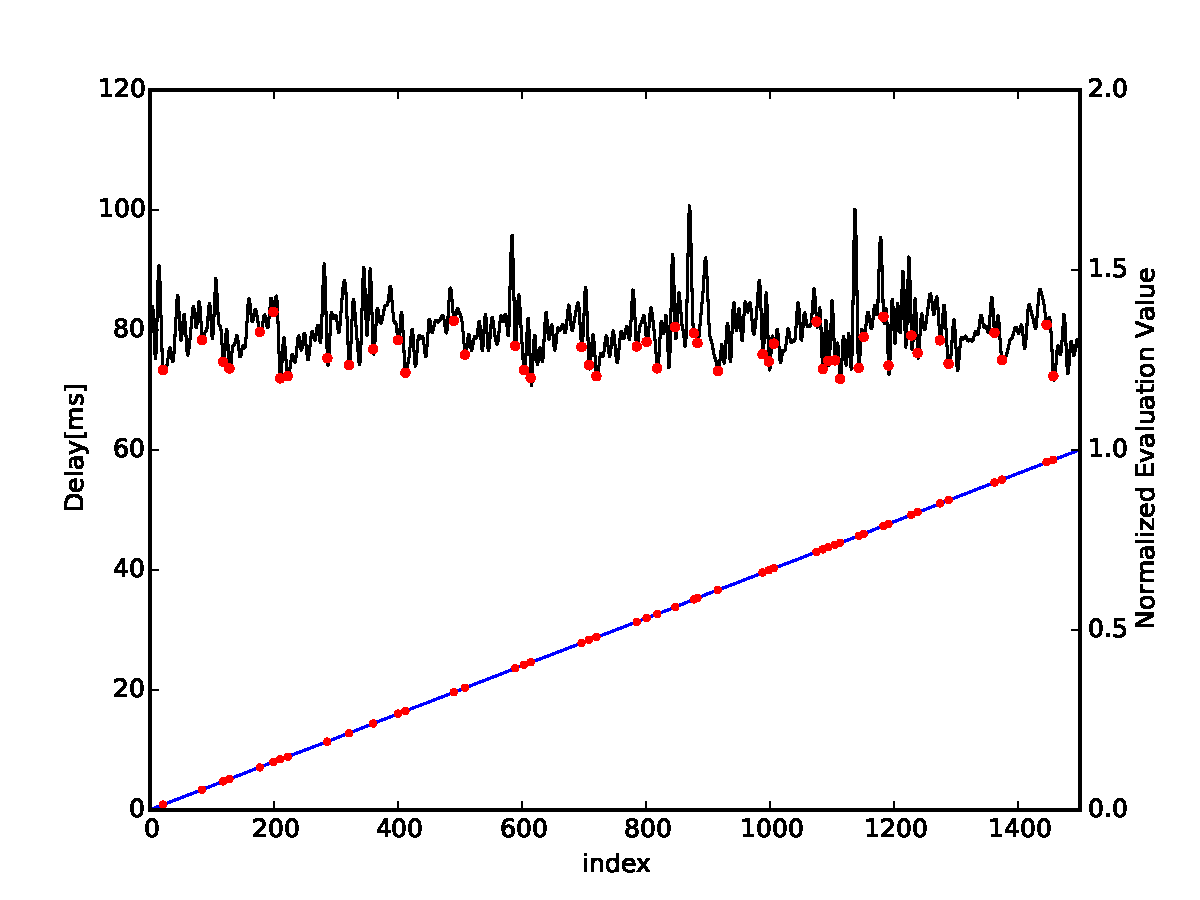
\includegraphics[width=0.5\hsize]{C:/master/mstudy/analysis/0829/result_integral_width20_alpha099.pdf}
}\\
\caption{手法 2 の実行結果($\alpha=0.99$)}
\label{resultalg2-2}
\end{center}
\end{figure}
図より,$\alpha$ が小さいほど全体の変曲点から分割点を制限して抽出できているが,図 \ref{resultalg2-1} のインデックス 500 付近に見られる明らかな分割点を抽出できていない.
このことから,$\alpha$ は 0.95 でも制限し過ぎであると考えられる.
また,この時に抽出されている分割点は単発的に発生する大きな応答遅延の影響を強く受けているように思える.
逆に$\alpha$ を 0.99 とすると変曲点から分割点をあまり制限できていない.
また,$l$ を大きくすると,分割点の直前に含まれる変曲点も抽出されるようになってしまっていた.
これは,変曲点直後の波の幅を長くしたことで,本来の分割点をまたぎ分割点を評価する式を計算しているためだと考えられる.
また,累積積分関数は変曲点が存在するもののほぼ直線に見える.
全体を通して安定して必要最小限の分割点を抽出することは困難であるように思われる.

\subsection{手法 3 : 統計量}
分割点の前後の直前の波形は直後の波形に比べて分布帯が大きい.
そこで一定区間幅における平均値や中央値といった統計量にこの差が表れるのではないかと予想し,これらに基づき抽出できないかを検討した.

\subsubsection{アルゴリズム}
統計量として平均値と中央値を用いる.
パラメータとして区間幅を表す $l$ を導入し,前処理後のデータを$x_i (i = 0,1,\ldots)$と表したとき,インデックス $j$ とそれより $l$ だけ前の区間に含まれるデータの平均値を表す $E_n$ とインデックス $j$ を中心として幅 $l$ の区間の中央値を表す $M_n$ は以下のように定まる.
$$E_n = \frac{1}{l} \sum^n_{k=n-l+1} x_k$$
$$M_n = Median\left(x_{n-\lfloor \frac{l}{2}\rfloor},\ldots,x_{n-1},x_n,x_{n+1},x_{n - \lfloor \frac{l}{2}\rfloor + l}\right)$$
$E_n$ や $M_n$ が急激に減少した箇所が分割点と考えられるため,パラメータ $\delta$ を用いて以下を満たすインデックス $n$ を分割点として抽出する.
$$E_{n-1} - E_n \geq \delta$$
$$M_{n-1} - M_n \geq \delta$$

\subsubsection{実行結果}
パラメータ $l$ と $\delta$ を変えながら平均値を用いて行った実行結果を図 \ref{resultalg3-1} から図 \ref{resultalg3-2} に示し,中央値を用いて行った実行結果を図 \ref{resultalg3-3} から図 \ref{resultalg3-4} に示す.
これらの図は黒線が前処理後の波形を示しており,青線は平均値を,緑線は中央値を示している.
また,赤点で黒線上に分割点を,青線や緑線上に分割点に対応する点を示した.
\begin{figure}[tb]
\begin{center}
\subfigure[$l = 5$]{
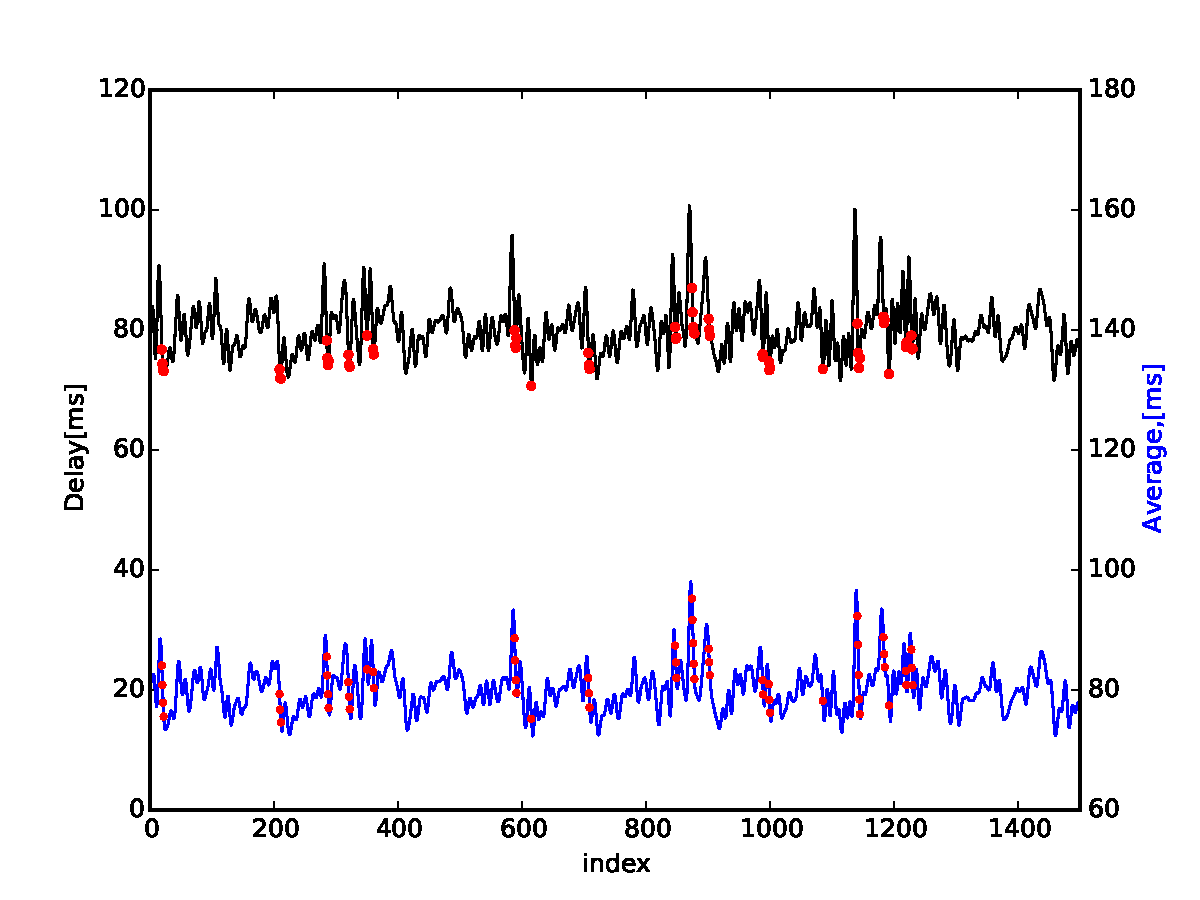
\includegraphics[width=0.5\hsize]{C:/master/mstudy/analysis/0829/result_average_width5_alpha2.pdf}
}~
\subfigure[$l = 10$]{
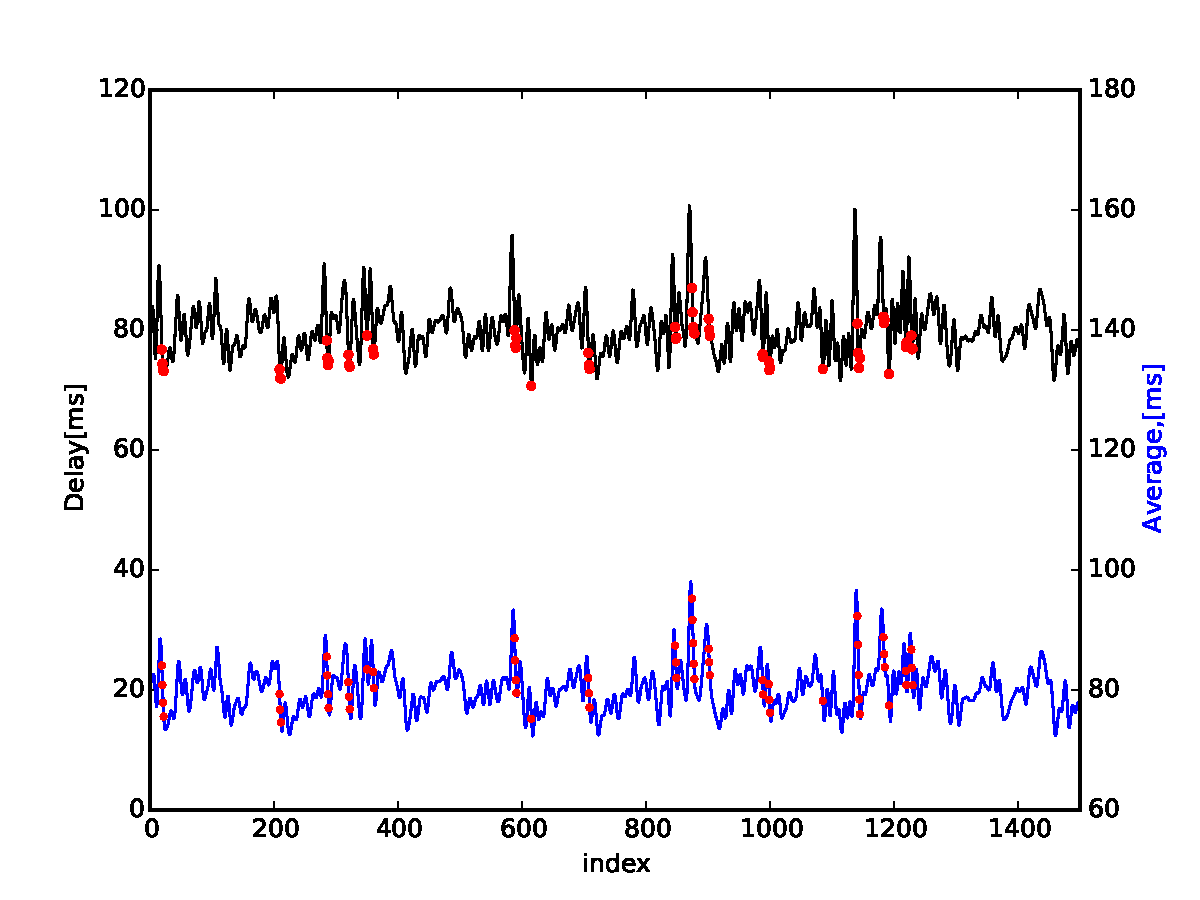
\includegraphics[width=0.5\hsize]{C:/master/mstudy/analysis/0829/result_average_width5_alpha2.pdf}
}\\
\subfigure[$l = 15$]{
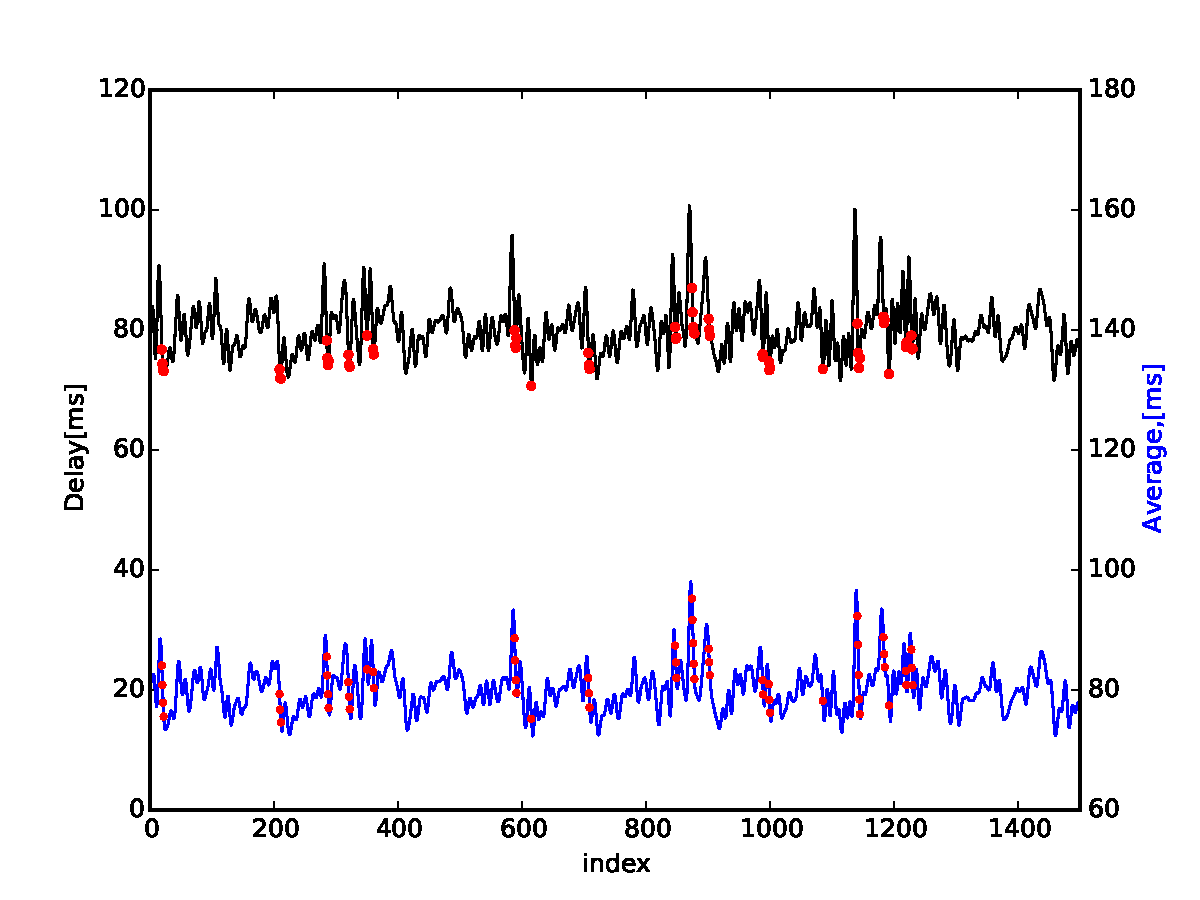
\includegraphics[width=0.5\hsize]{C:/master/mstudy/analysis/0829/result_average_width5_alpha2.pdf}
}~
\subfigure[$l = 20$]{
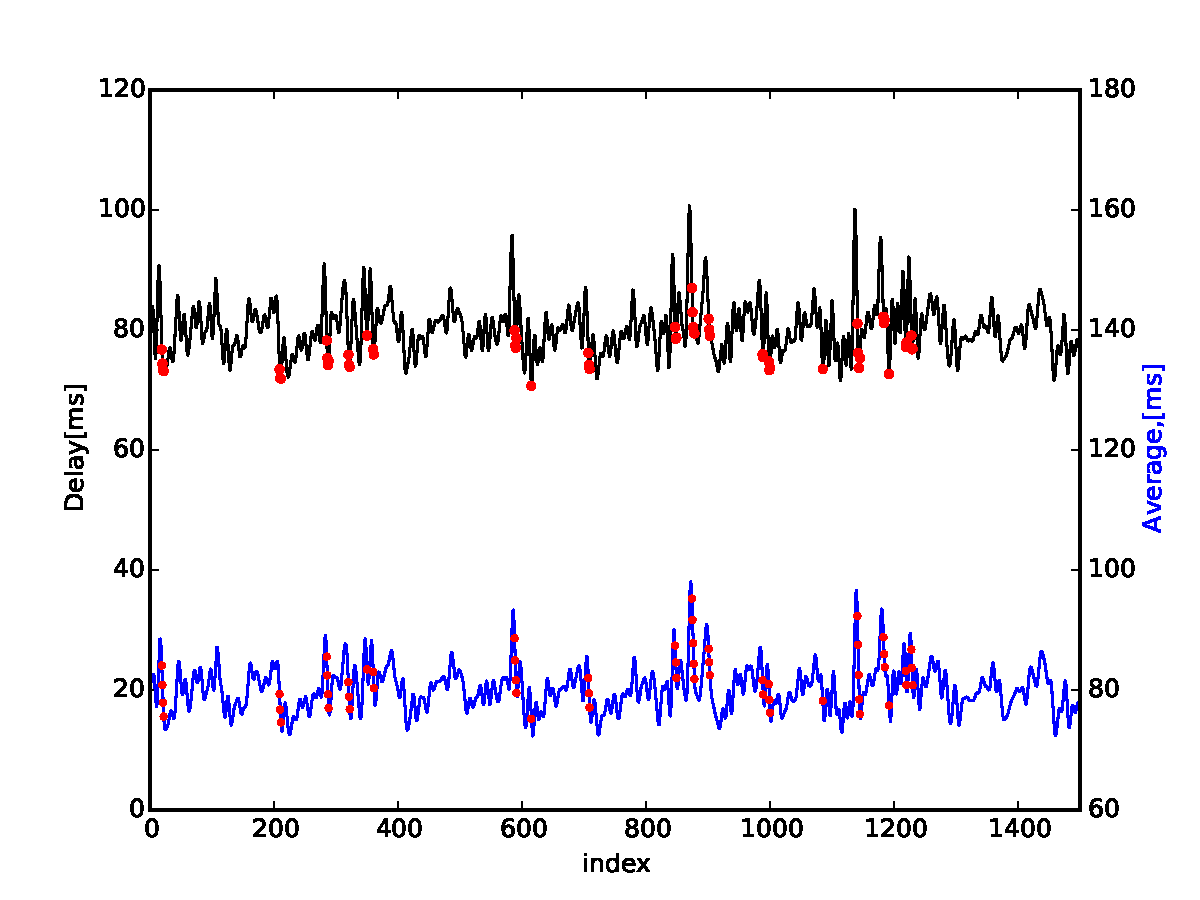
\includegraphics[width=0.5\hsize]{C:/master/mstudy/analysis/0829/result_average_width5_alpha2.pdf}
}\\
\caption{手法 3 の平均値を用いた実行結果($\delta = 2$)}
\label{resultalg3-1}
\end{center}
\end{figure}
\begin{figure}[tb]
\begin{center}
\subfigure[$l = 5$]{
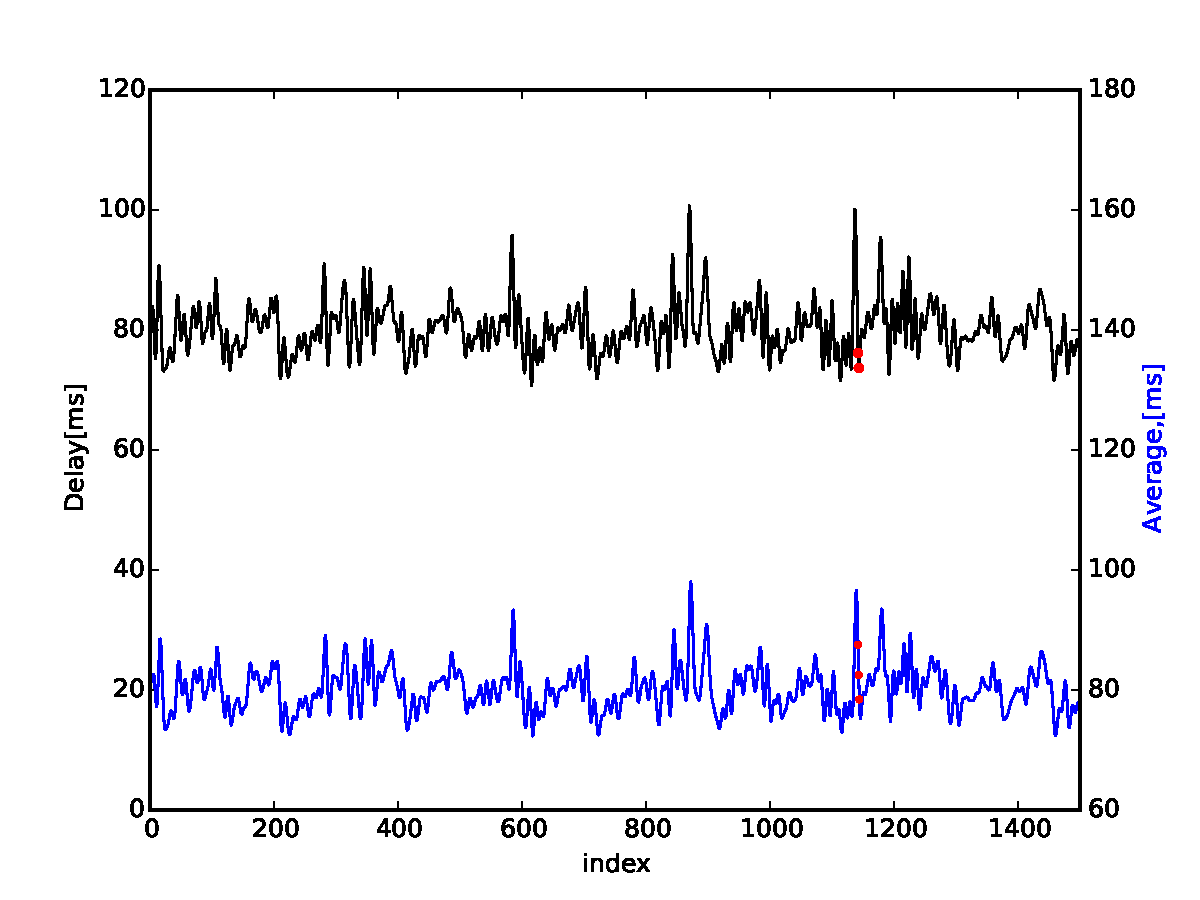
\includegraphics[width=0.5\hsize]{C:/master/mstudy/analysis/0829/result_average_width5_alpha4.pdf}
}~
\subfigure[$l = 10$]{
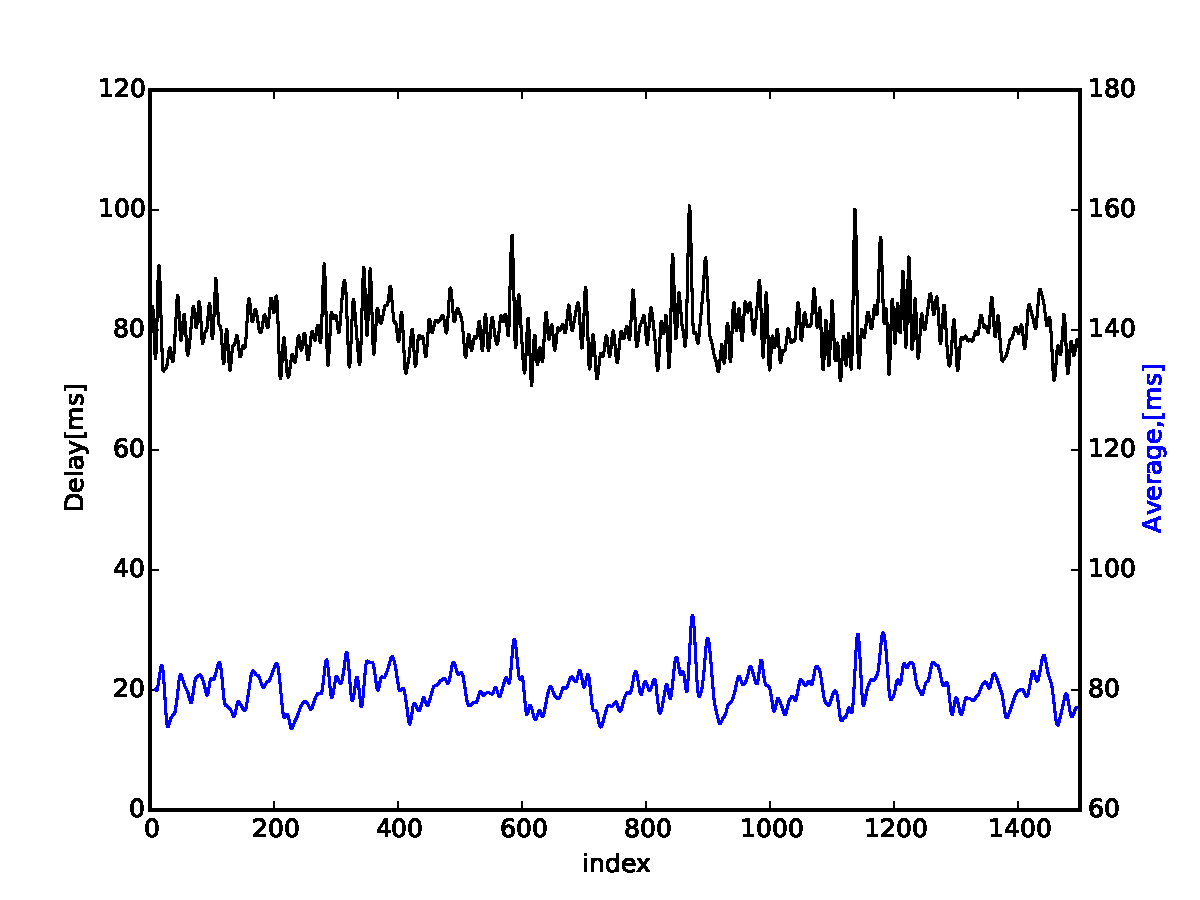
\includegraphics[width=0.5\hsize]{C:/master/mstudy/analysis/0829/result_average_width10_alpha4.pdf}
}\\
\subfigure[$l = 15$]{
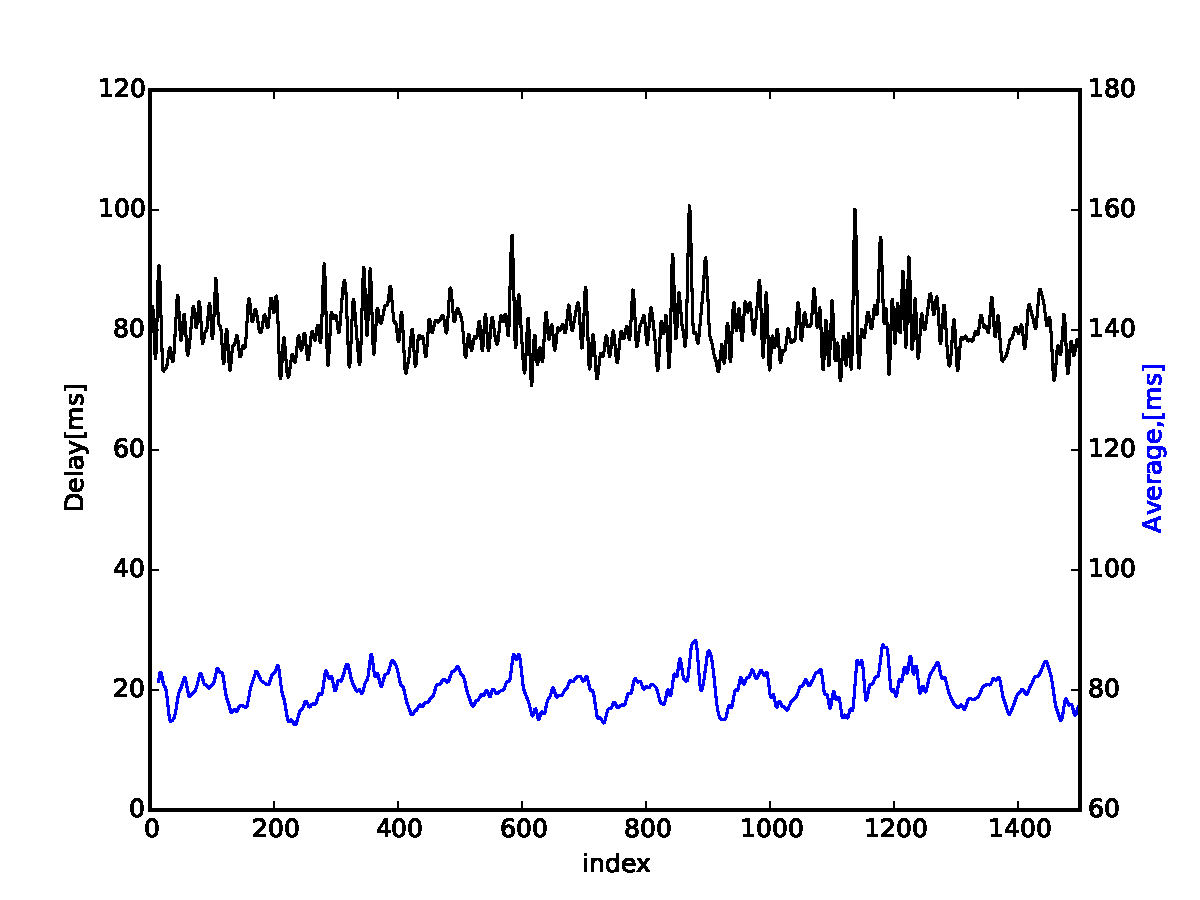
\includegraphics[width=0.5\hsize]{C:/master/mstudy/analysis/0829/result_average_width15_alpha4.pdf}
}~
\subfigure[$l = 20$]{
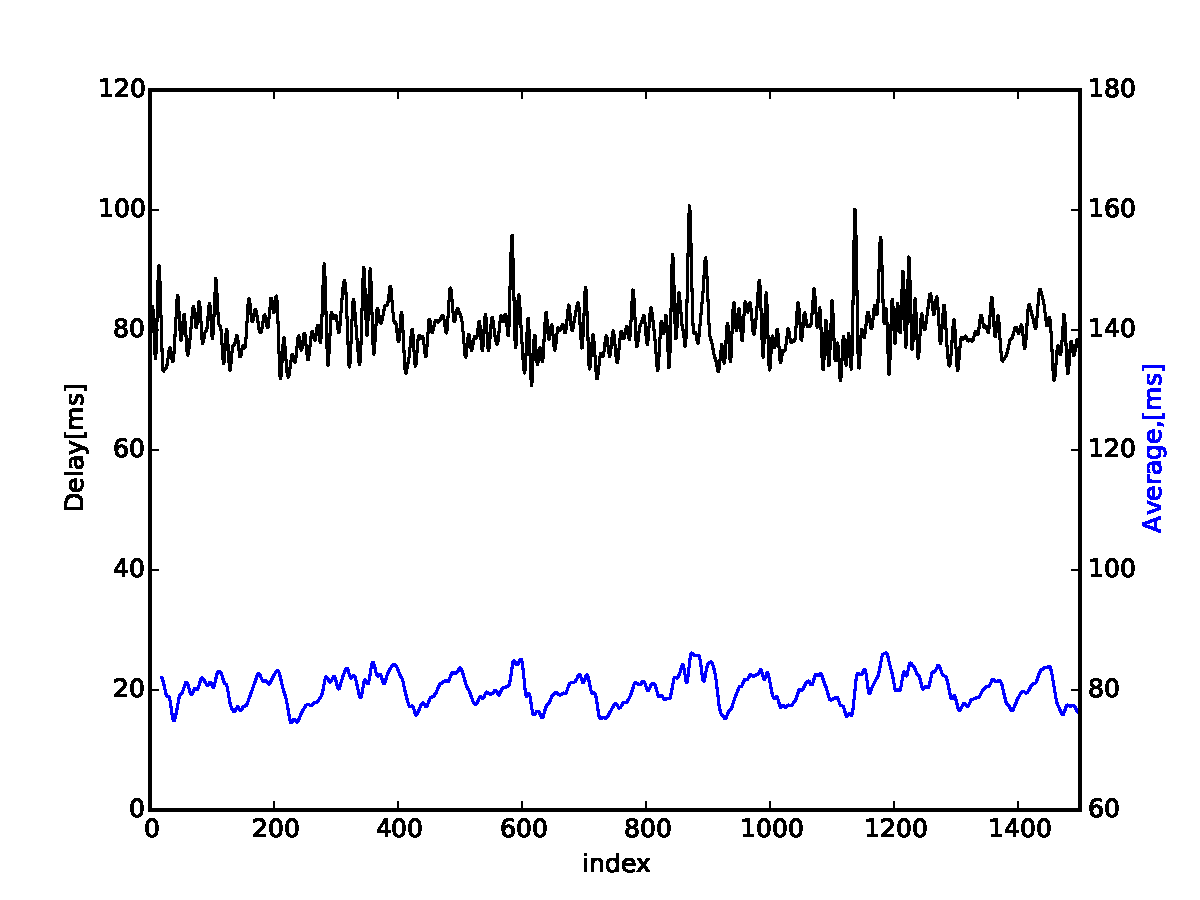
\includegraphics[width=0.5\hsize]{C:/master/mstudy/analysis/0829/result_average_width20_alpha4.pdf}
}\\
\caption{手法 3 の平均値を用いた実行結果($\delta = 4$)}
\end{center}
\end{figure}
\begin{figure}[tb]
\begin{center}
\subfigure[$l = 5$]{
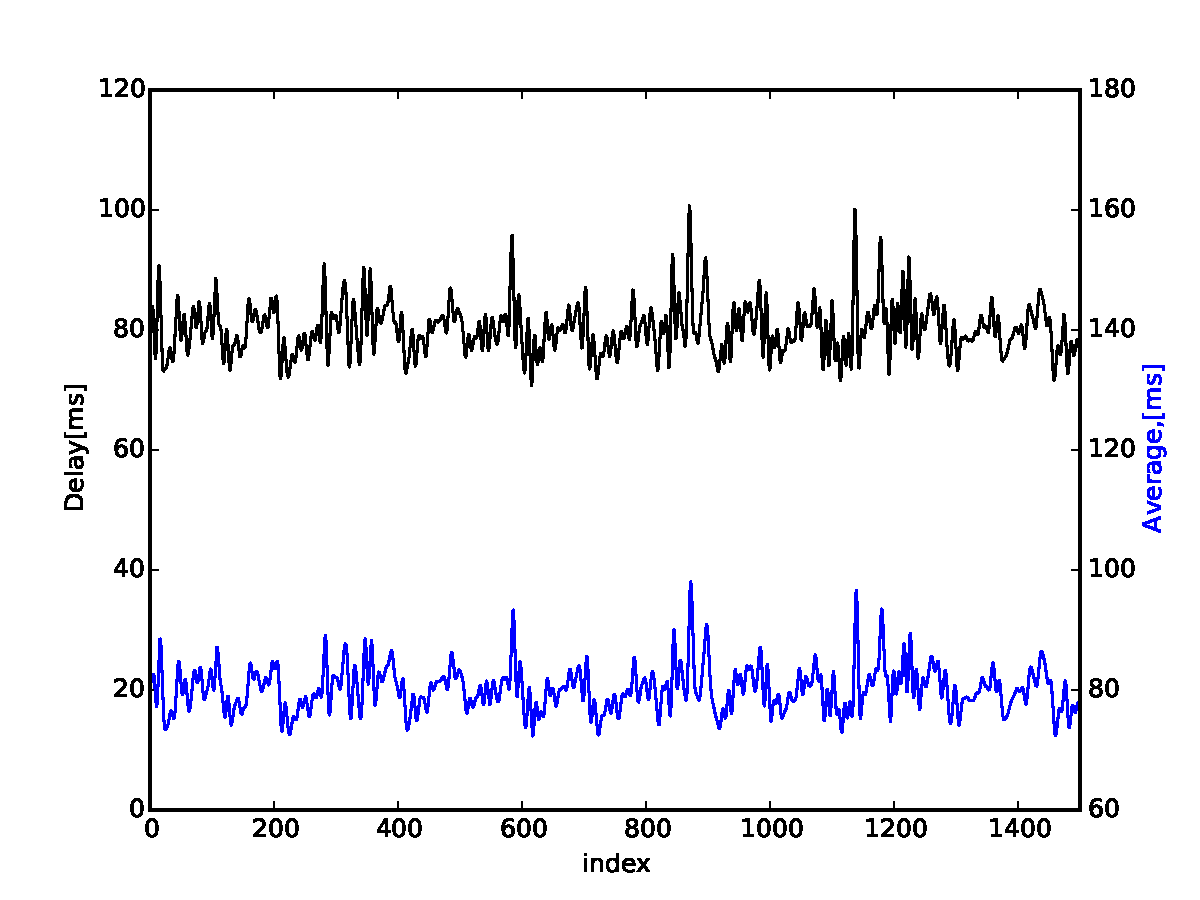
\includegraphics[width=0.5\hsize]{C:/master/mstudy/analysis/0829/result_average_width5_alpha6.pdf}
}~
\subfigure[$l = 10$]{
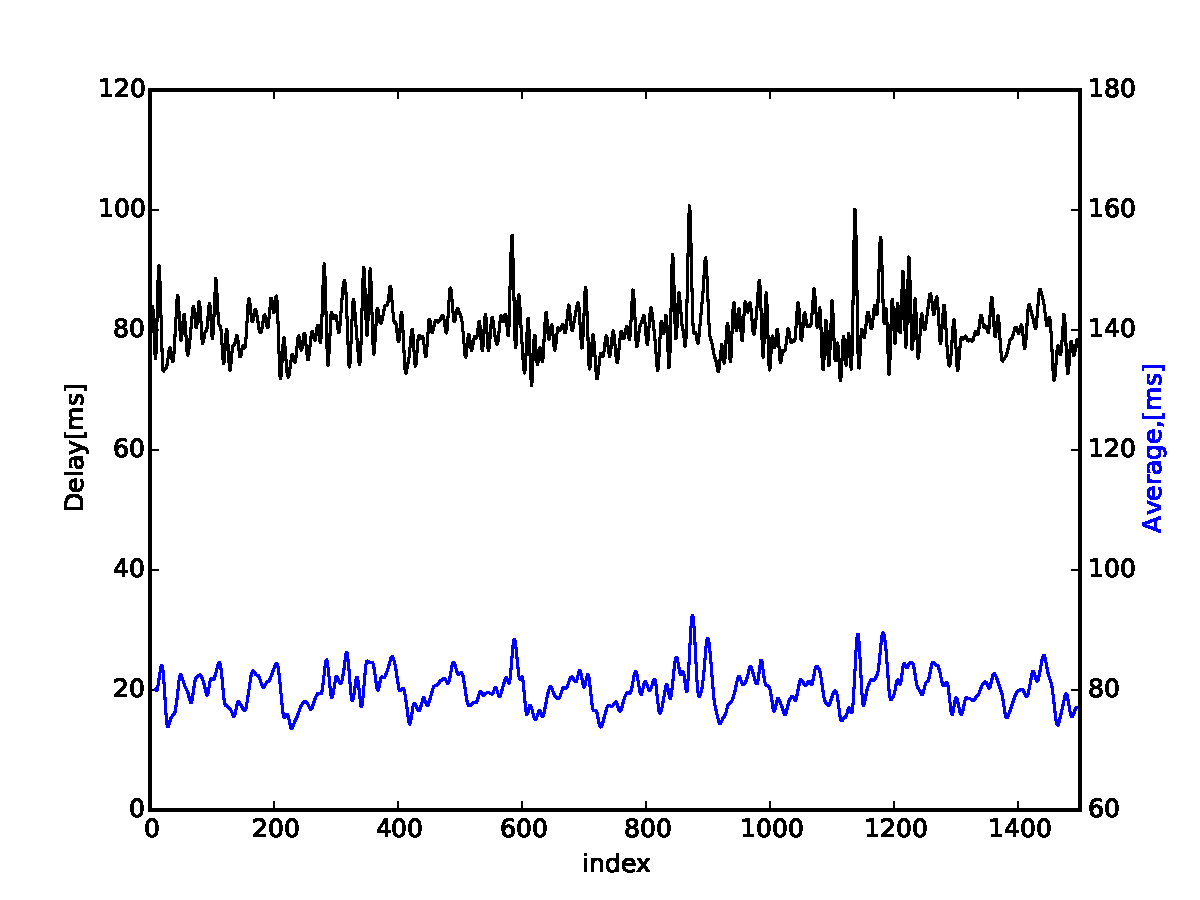
\includegraphics[width=0.5\hsize]{C:/master/mstudy/analysis/0829/result_average_width10_alpha6.pdf}
}\\
\subfigure[$l = 15$]{
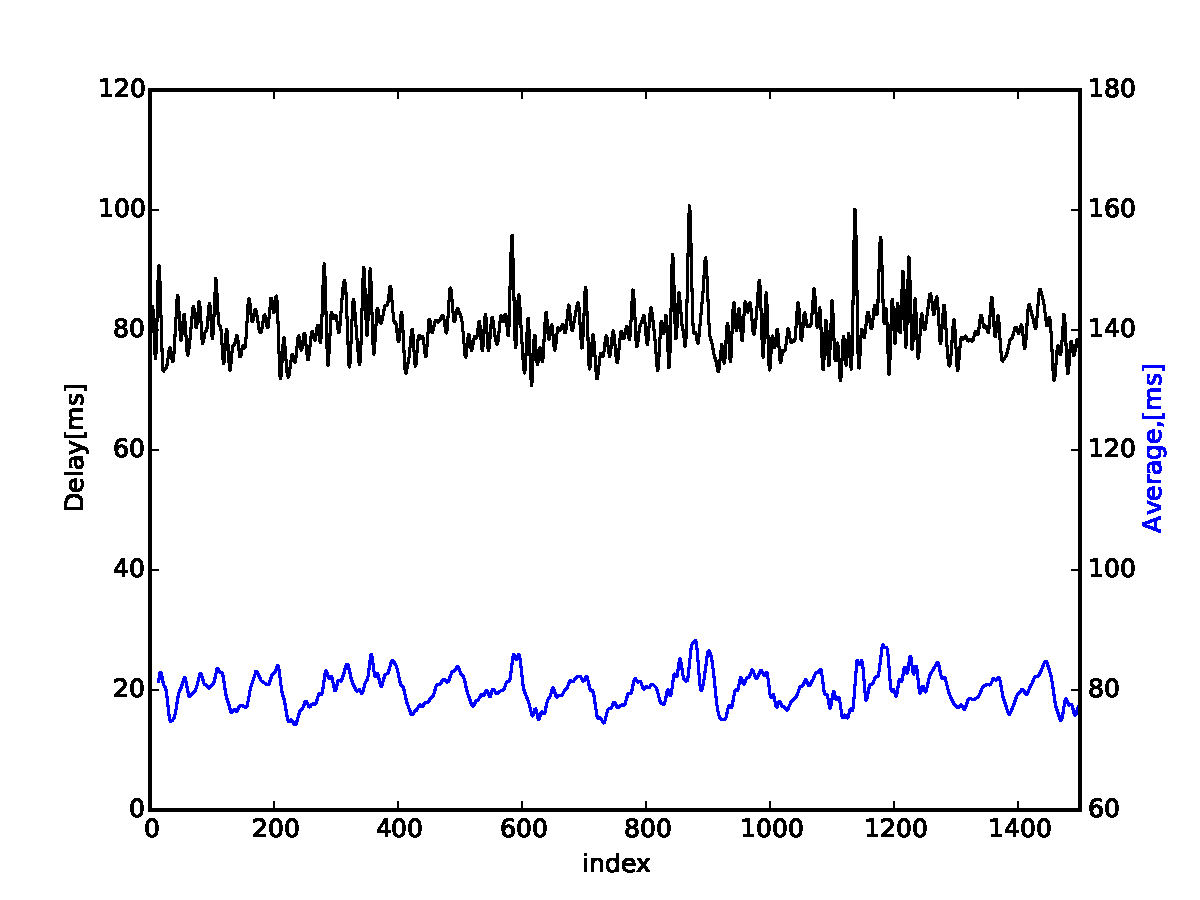
\includegraphics[width=0.5\hsize]{C:/master/mstudy/analysis/0829/result_average_width15_alpha6.pdf}
}~
\subfigure[$l = 20$]{
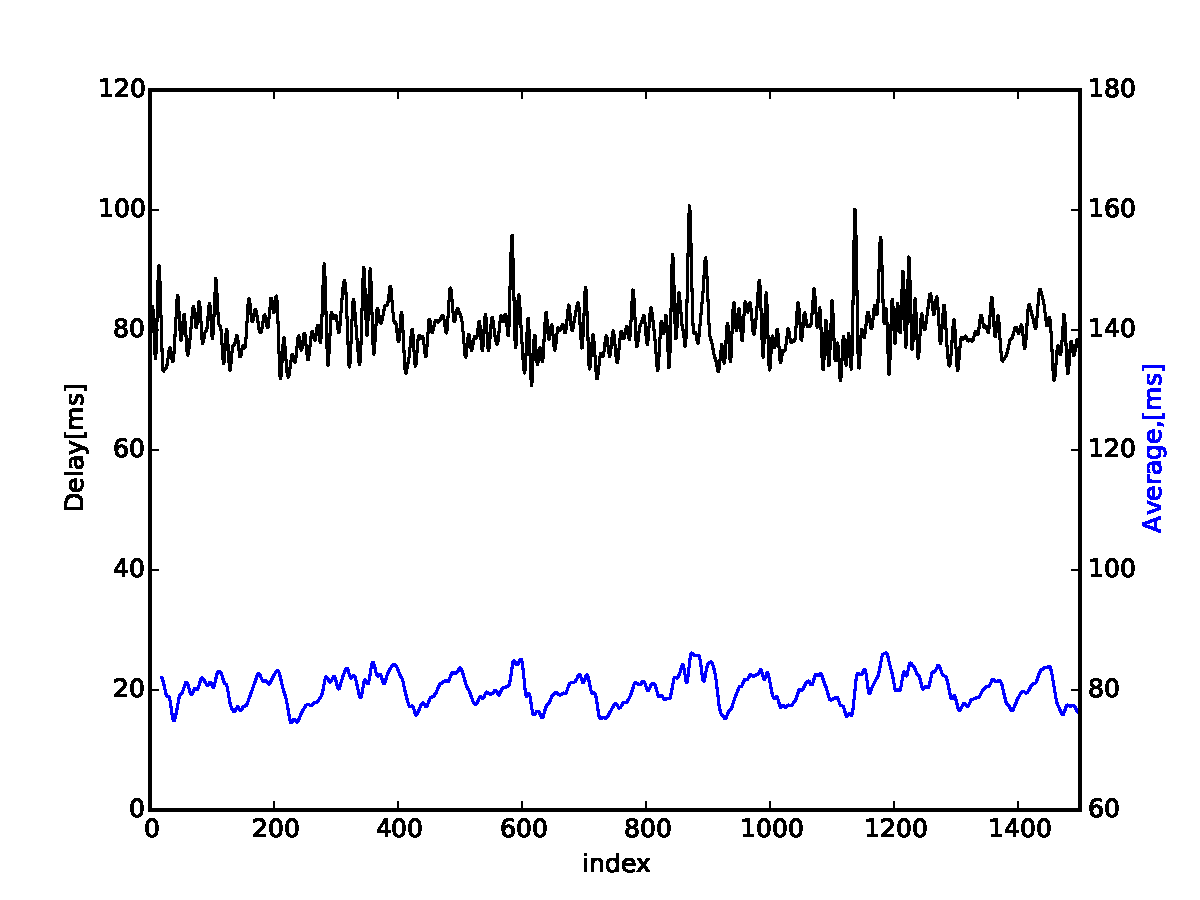
\includegraphics[width=0.5\hsize]{C:/master/mstudy/analysis/0829/result_average_width20_alpha6.pdf}
}\\
\caption{手法 3 の平均値を用いた実行結果($\delta = 6$)}
\label{resultalg3-2}
\end{center}
\end{figure}
\begin{figure}[tb]
\begin{center}
\subfigure[$l = 5$]{
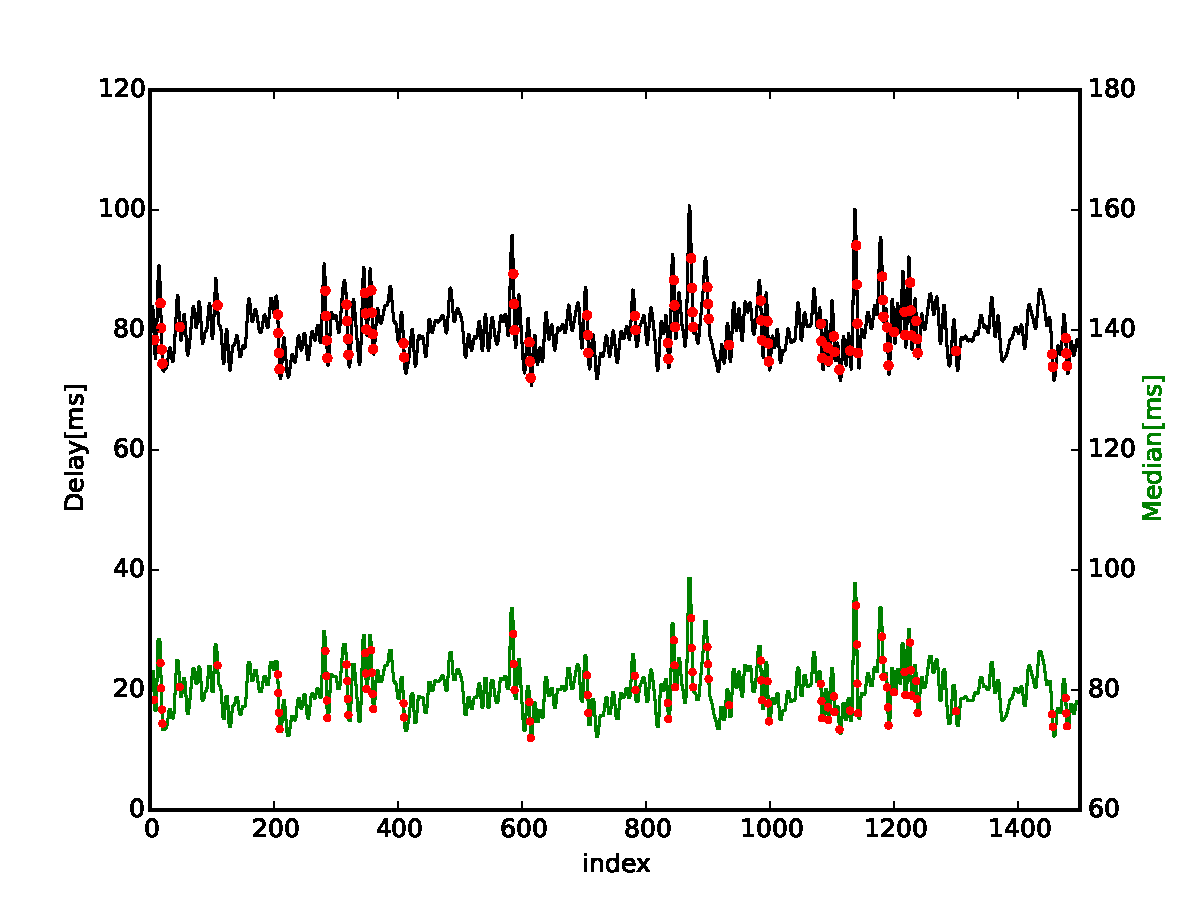
\includegraphics[width=0.5\hsize]{C:/master/mstudy/analysis/0829/result_median_width5_alpha2.pdf}
}~
\subfigure[$l = 10$]{
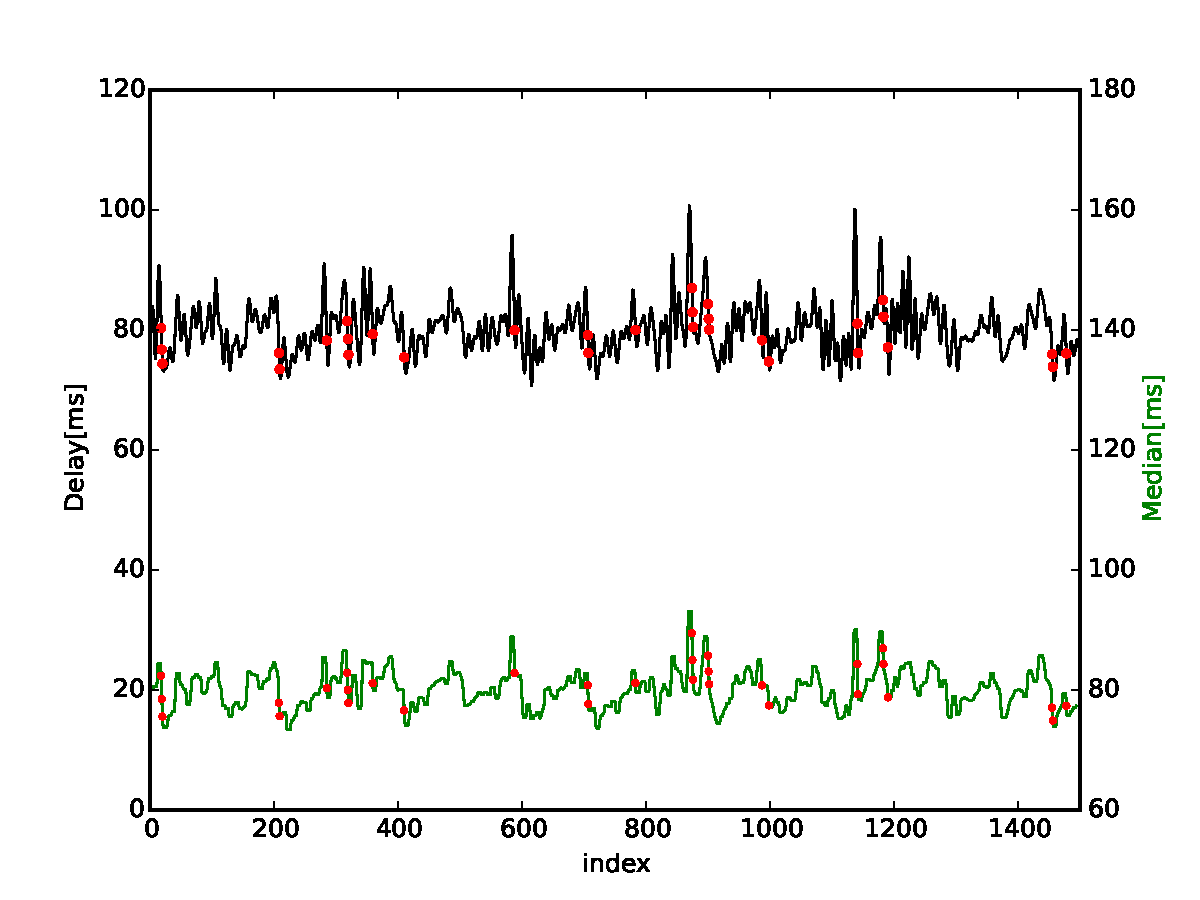
\includegraphics[width=0.5\hsize]{C:/master/mstudy/analysis/0829/result_median_width10_alpha2.pdf}
}\\
\subfigure[$l = 15$]{
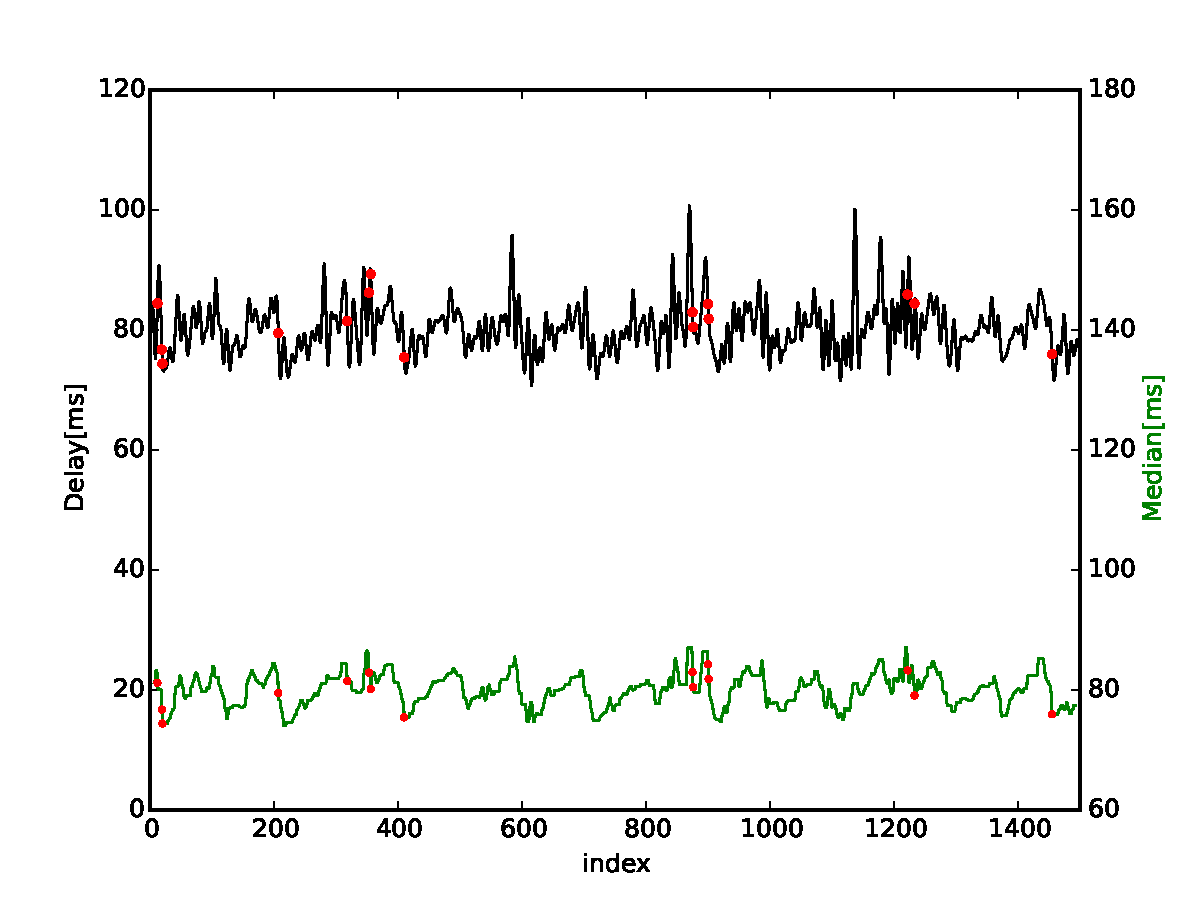
\includegraphics[width=0.5\hsize]{C:/master/mstudy/analysis/0829/result_median_width15_alpha2.pdf}
}~
\subfigure[$l = 20$]{
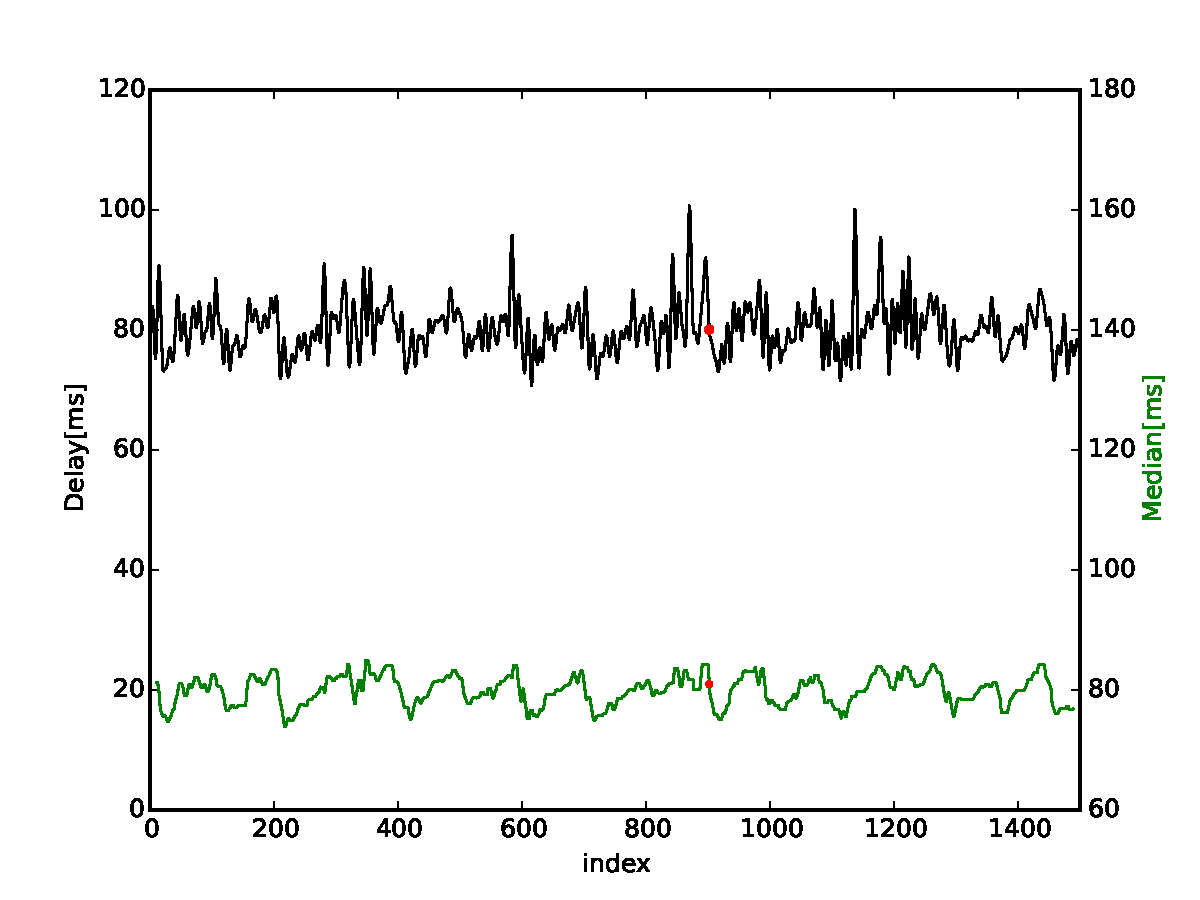
\includegraphics[width=0.5\hsize]{C:/master/mstudy/analysis/0829/result_median_width20_alpha2.pdf}
}\\
\caption{手法 3 の中央値を用いた実行結果($\delta = 2$)}
\label{resultalg3-3}
\end{center}
\end{figure}
\begin{figure}[tb]
\begin{center}
\subfigure[$l = 5$]{
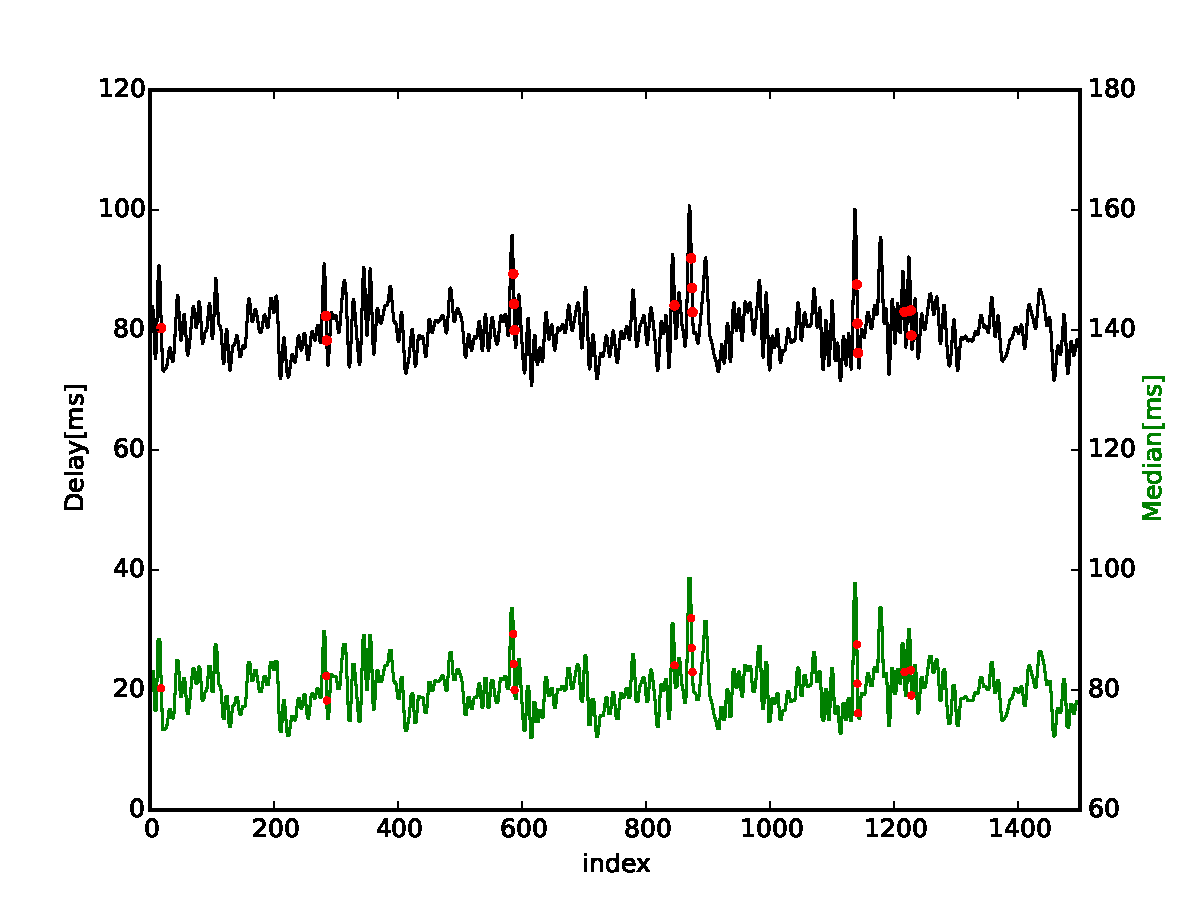
\includegraphics[width=0.5\hsize]{C:/master/mstudy/analysis/0829/result_median_width5_alpha4.pdf}
}~
\subfigure[$l = 10$]{
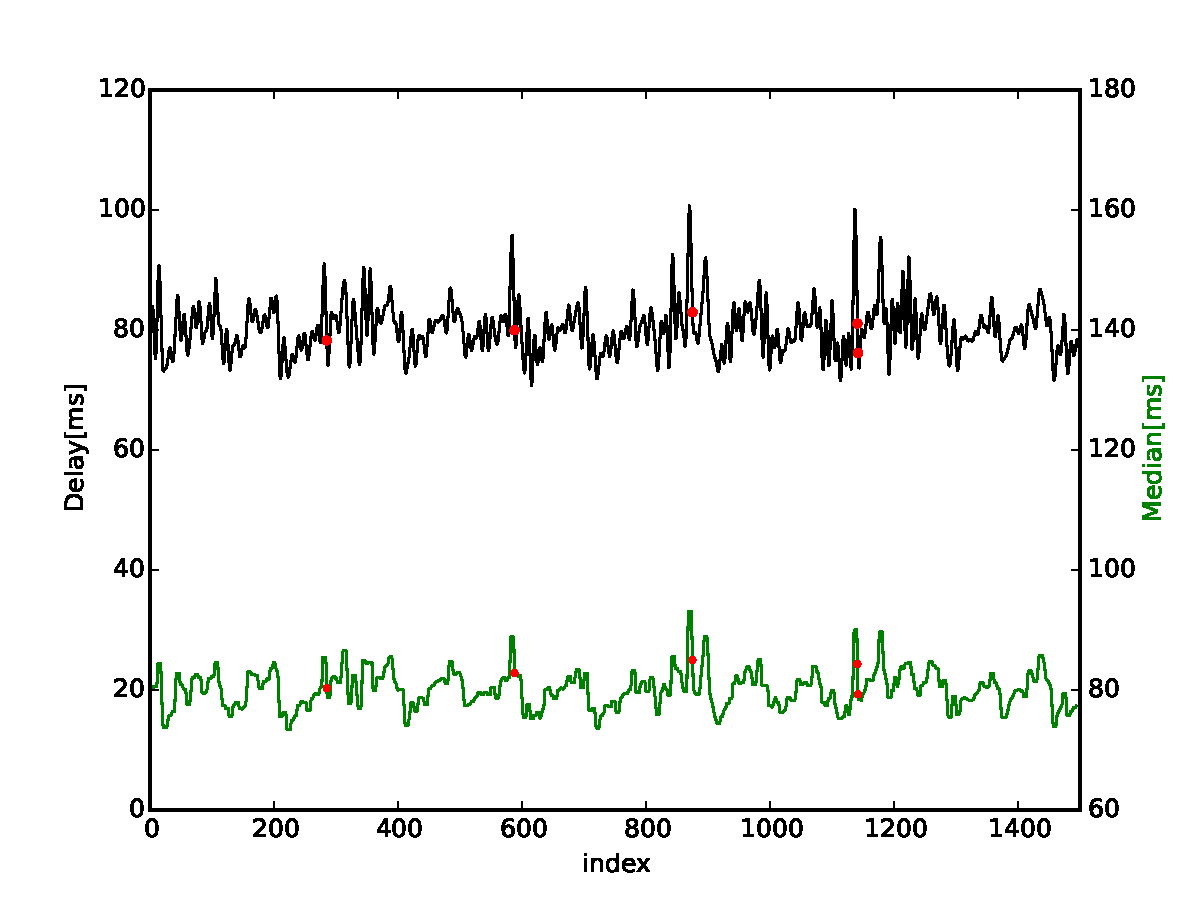
\includegraphics[width=0.5\hsize]{C:/master/mstudy/analysis/0829/result_median_width10_alpha4.pdf}
}\\
\subfigure[$l = 15$]{
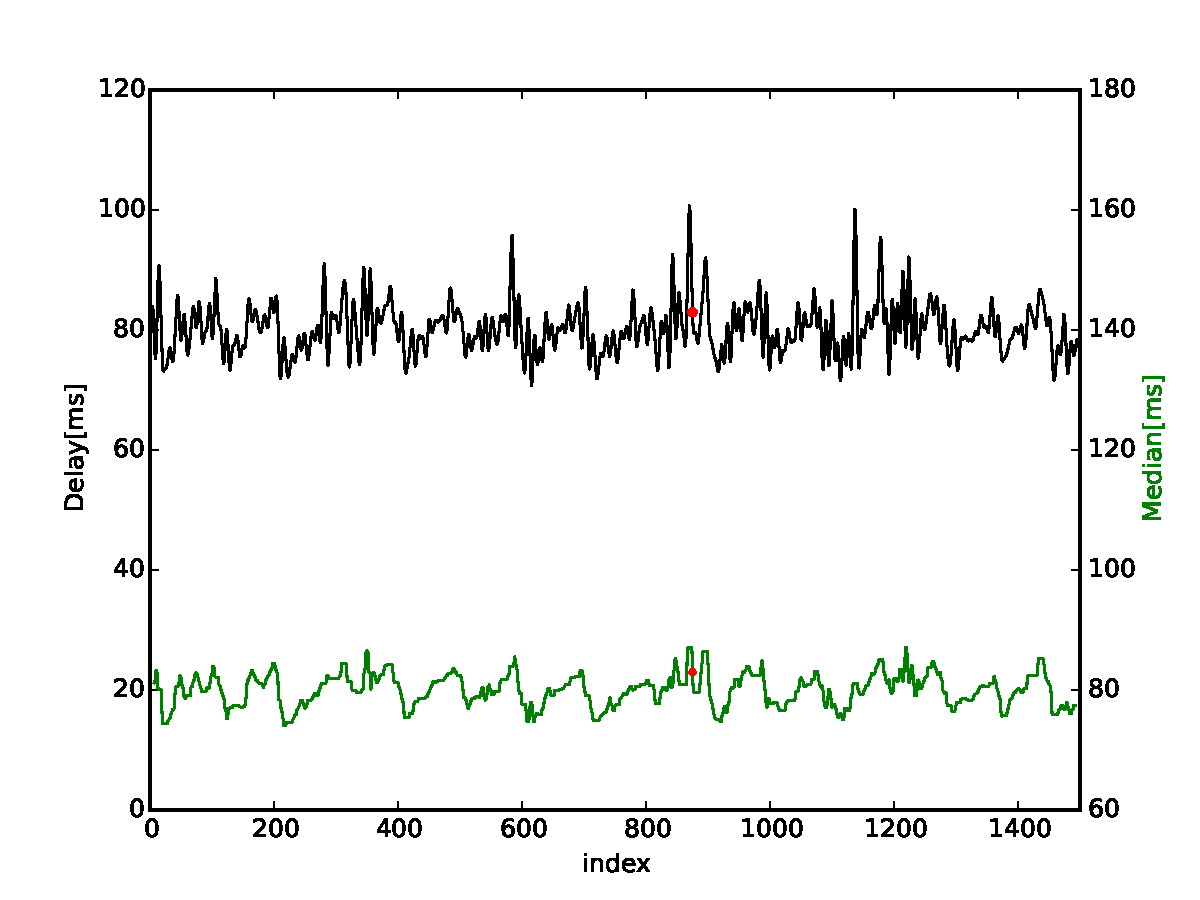
\includegraphics[width=0.5\hsize]{C:/master/mstudy/analysis/0829/result_median_width15_alpha4.pdf}
}~
\subfigure[$l = 20$]{
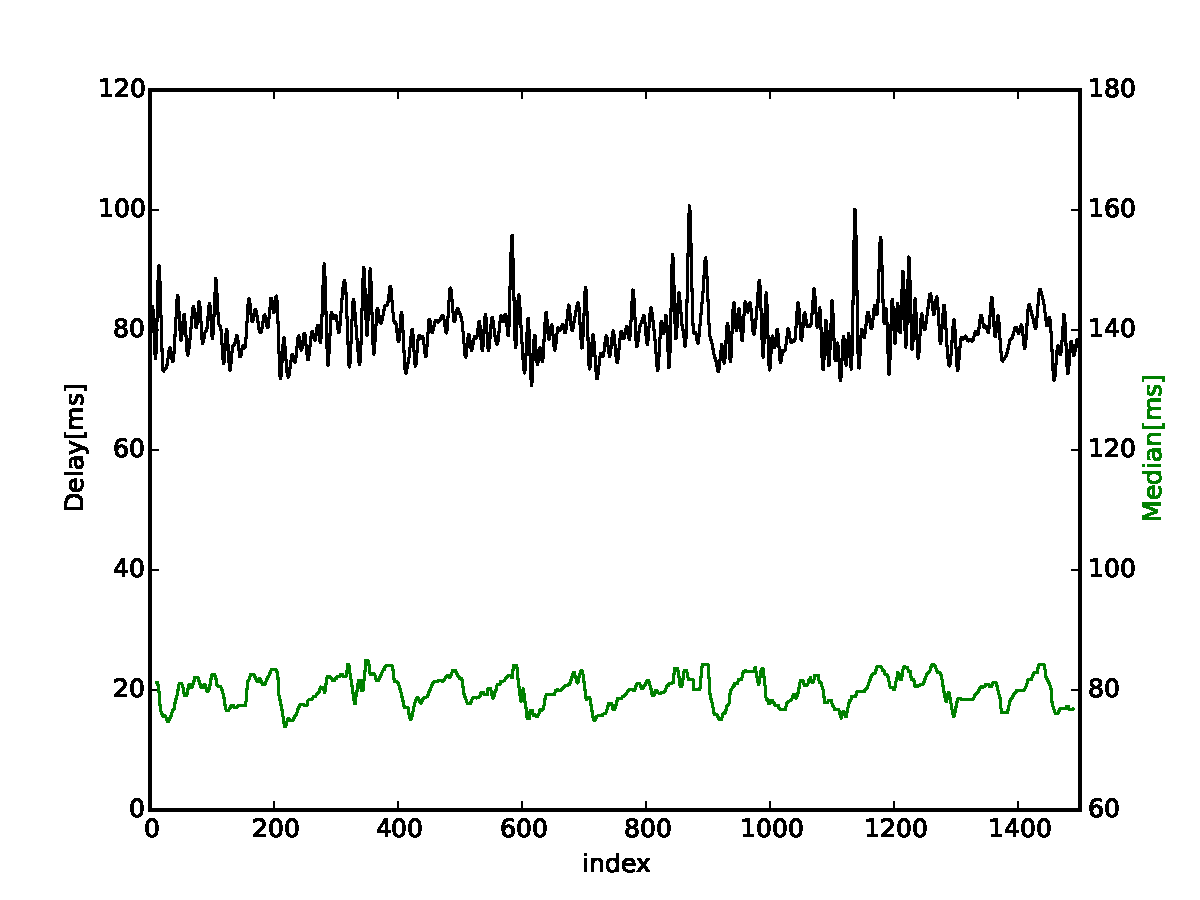
\includegraphics[width=0.5\hsize]{C:/master/mstudy/analysis/0829/result_median_width20_alpha4.pdf}
}\\
\caption{手法 3 の中央値を用いた実行結果($\delta = 4$)}
\end{center}
\end{figure}
\begin{figure}[tb]
\begin{center}
\subfigure[$l = 5$]{
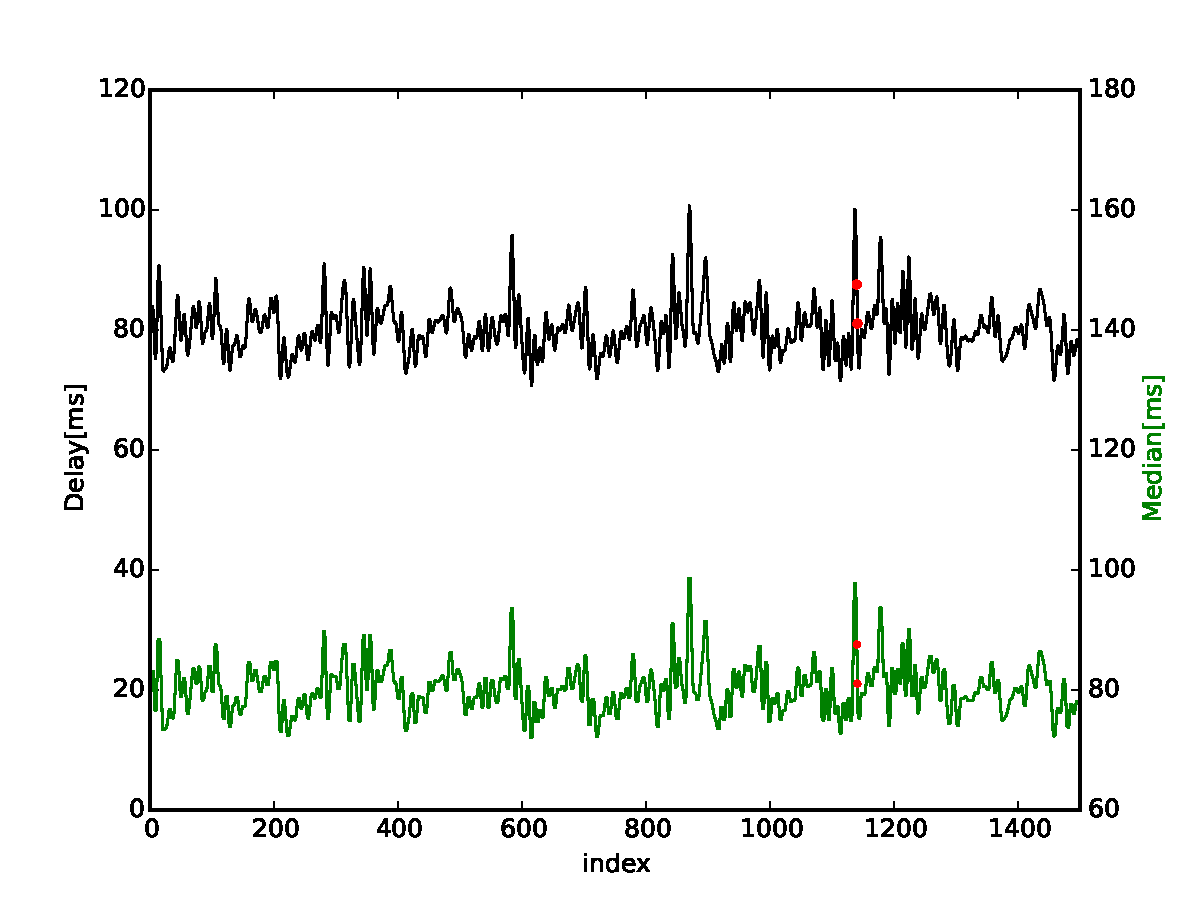
\includegraphics[width=0.5\hsize]{C:/master/mstudy/analysis/0829/result_median_width5_alpha6.pdf}
}~
\subfigure[$l = 10$]{
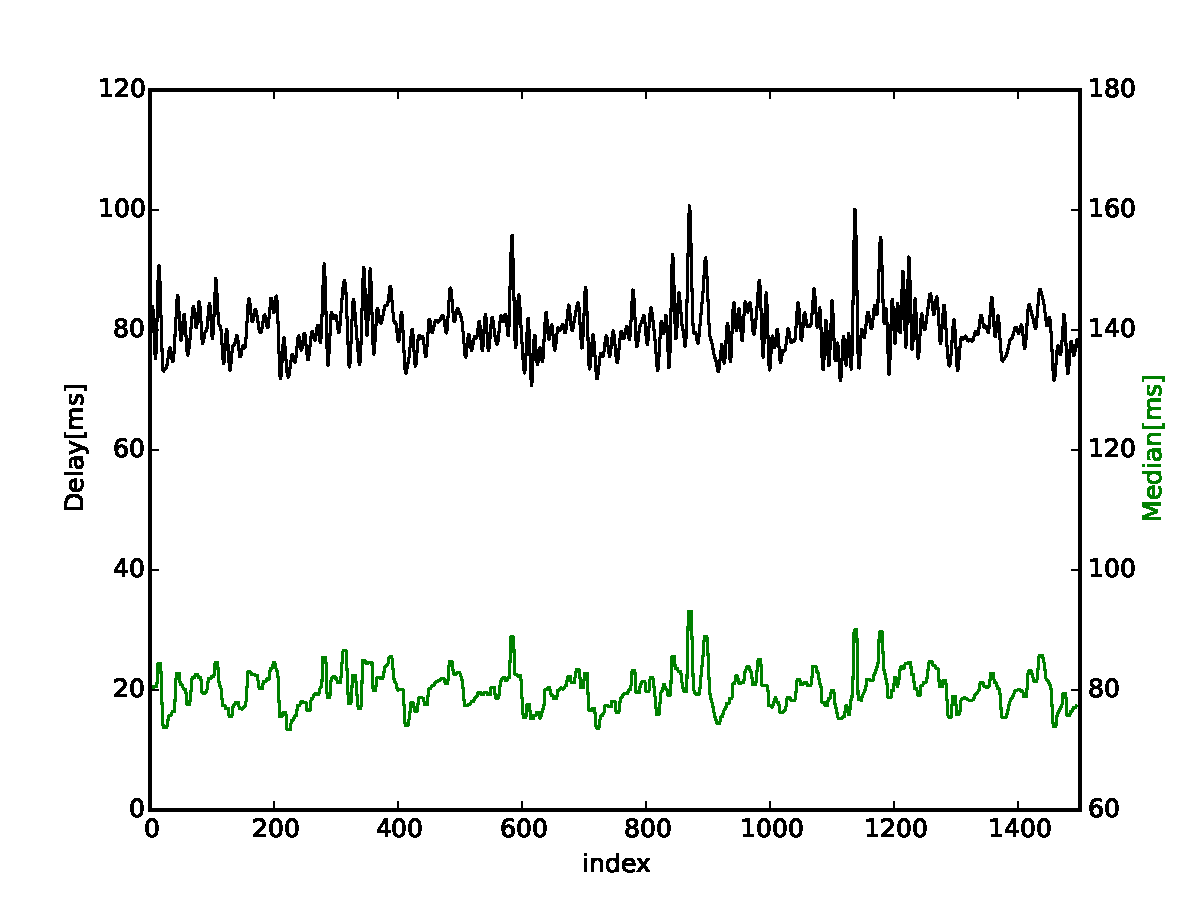
\includegraphics[width=0.5\hsize]{C:/master/mstudy/analysis/0829/result_median_width10_alpha6.pdf}
}\\
\subfigure[$l = 15$]{
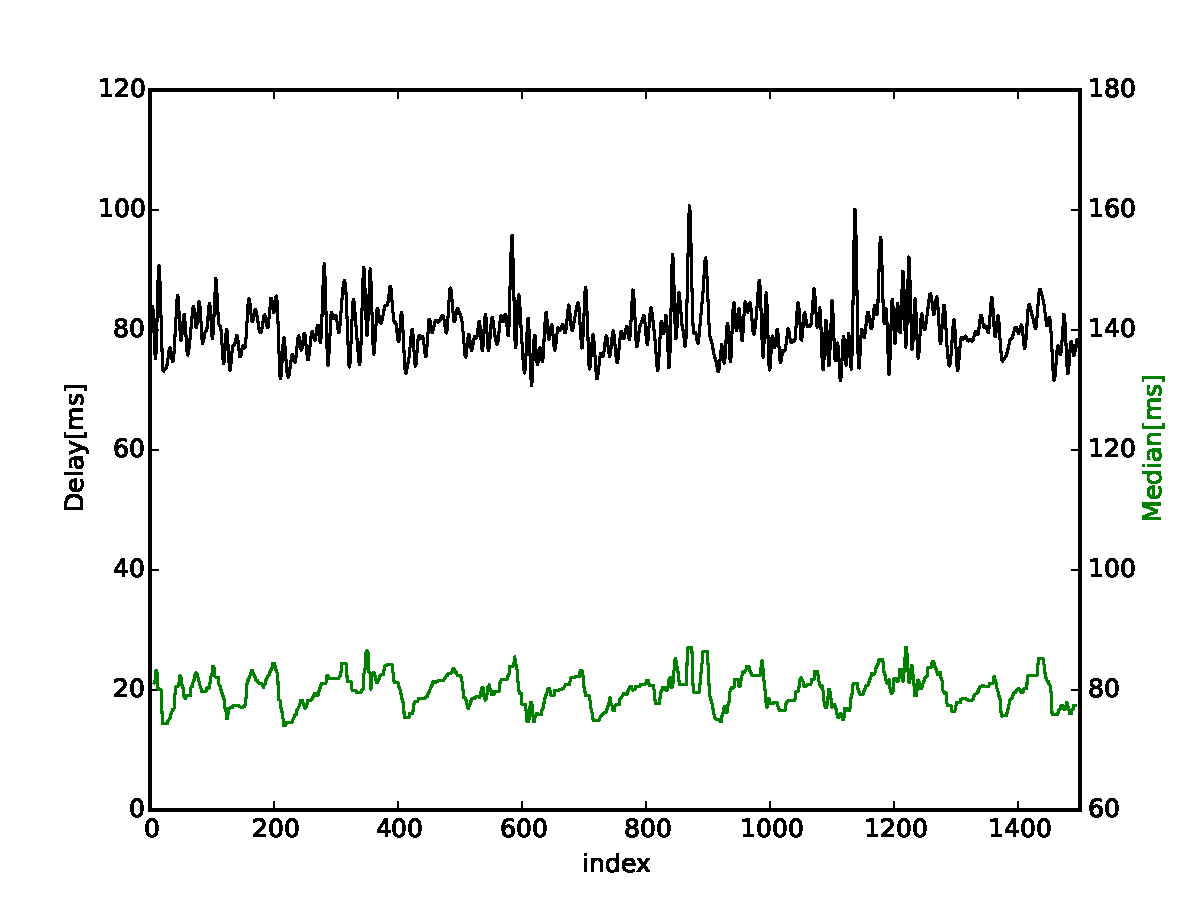
\includegraphics[width=0.5\hsize]{C:/master/mstudy/analysis/0829/result_median_width15_alpha6.pdf}
}~
\subfigure[$l = 20$]{
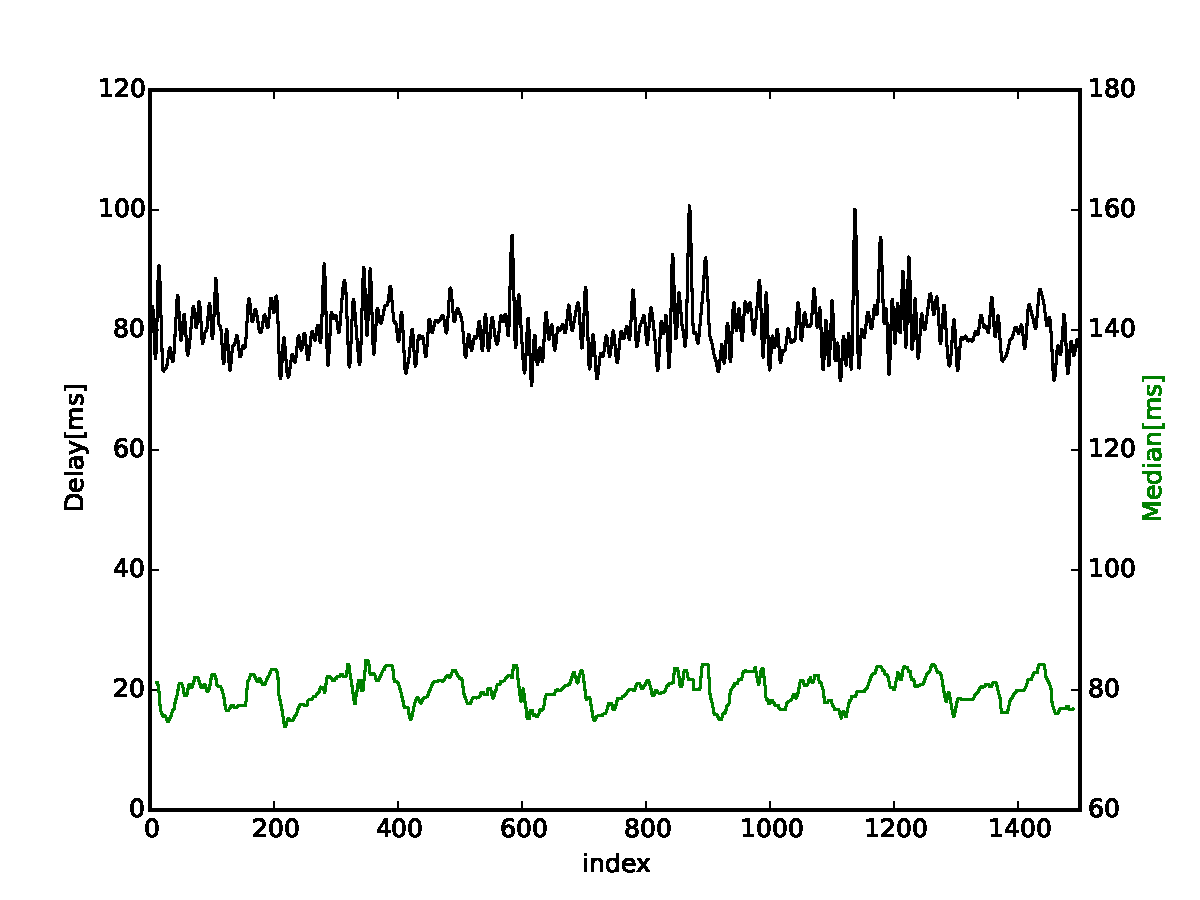
\includegraphics[width=0.5\hsize]{C:/master/mstudy/analysis/0829/result_median_width20_alpha6.pdf}
}\\
\caption{手法 3 の中央値を用いた実行結果($\delta = 6$)}
\label{resultalg3-4}
\end{center}
\end{figure}

図より,平均値では望ましい分割点が得られる場合があるものの,その近傍から多くの分割点を合わせて抽出してしまっている.
これは近い区間幅に含まれる波の平均値は近い値となることにより,分割点周辺のいくつかの点では分割点と似た振る舞いをするためだと思われる.
また,中央値では分割点でない点が抽出されることが多いようだ.
これは中央値ではインデックスの大小関係を考慮しないため,連続する二つのインデックス間で値が急減する分割点を正確に抽出することができなかったと考えられる.
また,平均値や中央値のどちらにおいても前処理後の波形をさらに平滑化したものが得られているため,用いるとしても抽出手法というよりは前処理の手法の方が適しているように感じた.

\subsection{手法 4 : 回帰直線の傾きの連続的な減少}
のこぎり波の開始点から区間を増加させながら逐次的に単回帰を行う場合,分割点直後の波形は一概に回帰線を下回るため,回帰直線の傾きは連続して減少していくと考えられる.
そこで,回帰直線の傾きが連続して減少し始めた時点を分割点として抽出できないかを検討した.

\subsubsection{アルゴリズム}
インデックス 0 を開始点として少なくともインデックス幅が 20 以上となる各区間のそれぞれに対して最小二乗法により単回帰を行い,それらの傾きを求める.
この時,傾きが $l$ 区間幅の間連続して減少した場合,この減少の開始時点を分割点として抽出する.

\subsubsection{実行結果}
パラメータ $l$ を変えながら実行した結果を図 \ref{resultalg4} に示す.
これらの図は黒線が前処理後の波形を示しており,色線は分割点で分割された各区間の波形の回帰直線である.
また,右側の縦軸には開始点から横軸のインデックスまでの区間の回帰直線の傾きを取っており,アルゴリズム実行中において各色の回帰直線の終了時点に当たる分割点を求める際の傾きの値を回帰直線と同色で示した.
\begin{figure}[tb]
\begin{center}
\subfigure[$l = 15$]{
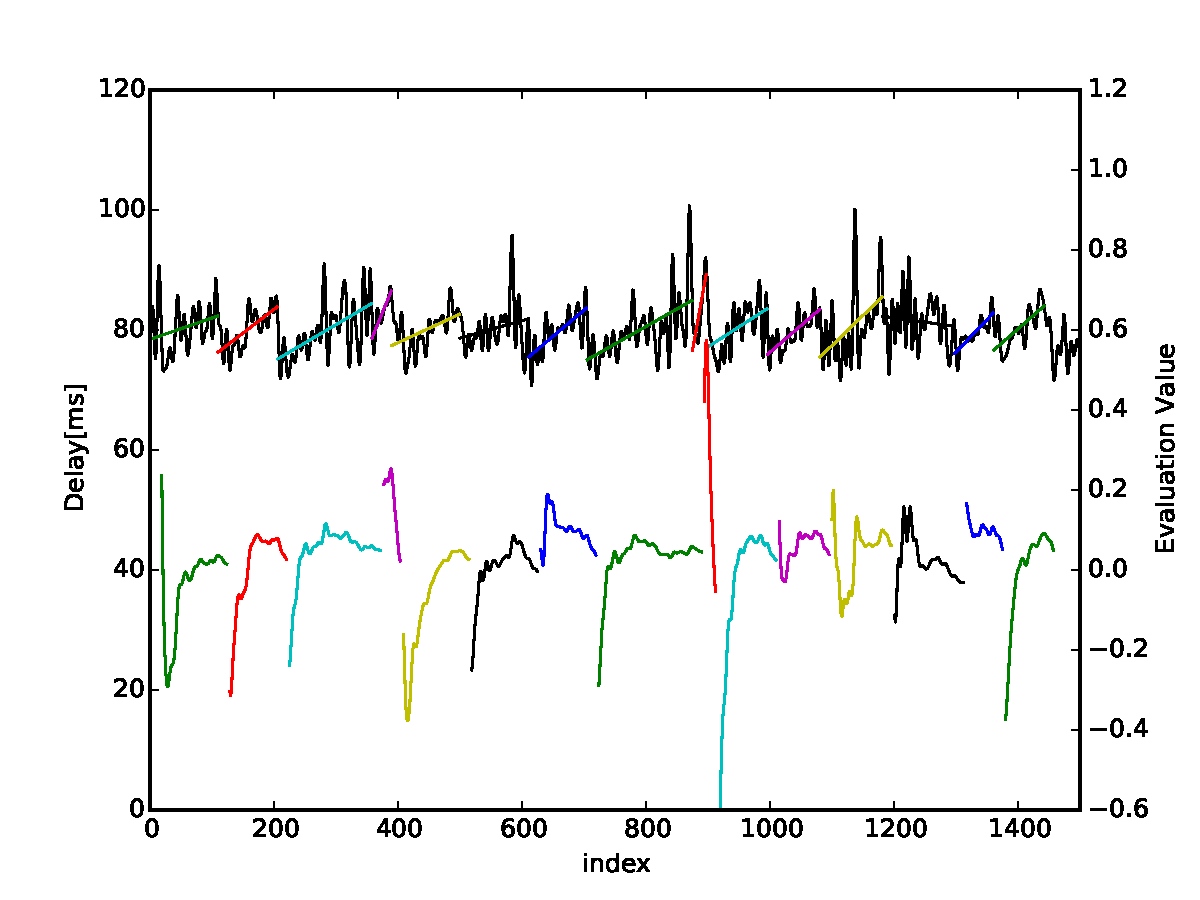
\includegraphics[width=0.9\hsize]{C:/master/mstudy/analysis/0829/result_decline_width15.pdf}
}\\
\subfigure[$l = 20$]{
\includegraphics[width=0.9\hsize]{C:/master/mstudy/analysis/0829/result_decline_width20.pdf}
}
\end{center}
\end{figure}
\begin{figure}[tb]
\begin{center}
\subfigure[$l = 25$]{
\includegraphics[width=0.9\hsize]{C:/master/mstudy/analysis/0829/result_decline_width25.pdf}
}
\caption{手法 4 の実行結果}
\label{resultalg4}
\end{center}
\end{figure}

\subsection{手法 5 : シャープネスを変化させたときの変化量}
時間が足りなかったため未実施です.
\end{document}